\documentclass[12pt]{article}

\usepackage{color}
\usepackage{hyperref}

\usepackage{amsmath}
\usepackage{amssymb}

\usepackage{geometry}
\geometry{a4paper}

\usepackage{graphicx}
\graphicspath{%
{figures/checks/}
{figures/efficiency/}
{figures/syst/}}
%%%%%%%%%%%%%%%%%%%%%%%%%%%%%%

\newcommand{\emp}[1]{\textcolor{magenta}{#1}}

\newcommand{\conc}[1]{\emp{\textbf{Conclusion:} #1}}

\newcommand{\emplist}[3]{%
\begin{description}
\item[\textcolor{red}{[L.~#1, p.~#2]}] \textcolor{red}{#3}
\end{description}}

\newcommand{\cent}[2]{$#1$--$#2\%$}
\newcommand{\pT}{\ensuremath{p_{\rm T}}}

\newcommand{\Vzero}{\ensuremath{{\rm V}^{0}}}
\newcommand{\Kshort}{\ensuremath{{\rm K}_{\rm S}^{0}}}
\newcommand{\AntiLa}{\ensuremath{\overline{\Lambda}}}
%%%%%%%%%%%%%%%%%%%%%%%%%%%%%%

\title{$\Lambda$ and $\Kshort$ production in jets in p--Pb collisions -- Support document}
\author{PC members}
%\date{}
%%%%%%%%%%%%%%%%%%%%%%%%%%%%%%

\begin{document}

\maketitle
%%%%%%%%%%%%%%%%%%%%%%%%%%%%%%

\section*{Todo}

\begin{itemize}
\item The reply of comments at \emp{[L.~175, p.~5]}.
\item Update of the systematic uncertainty.
\end{itemize}
%%%%%%%%%%%%%%%%%%%%%%%%%%%%%%

\section{ Response of inline comments}

\emplist{175}{5}{MP: Sentence added on req. by Jana: �add a description how the $\Lambda$ and $\Kshort$ sample is clean after topological selection� $\Rightarrow$ check number -- extract from the invariant mass for the lowest $\pT$ bin considered -- $0.5$~GeV/$c$.}

\begin{figure}[h]
\centering
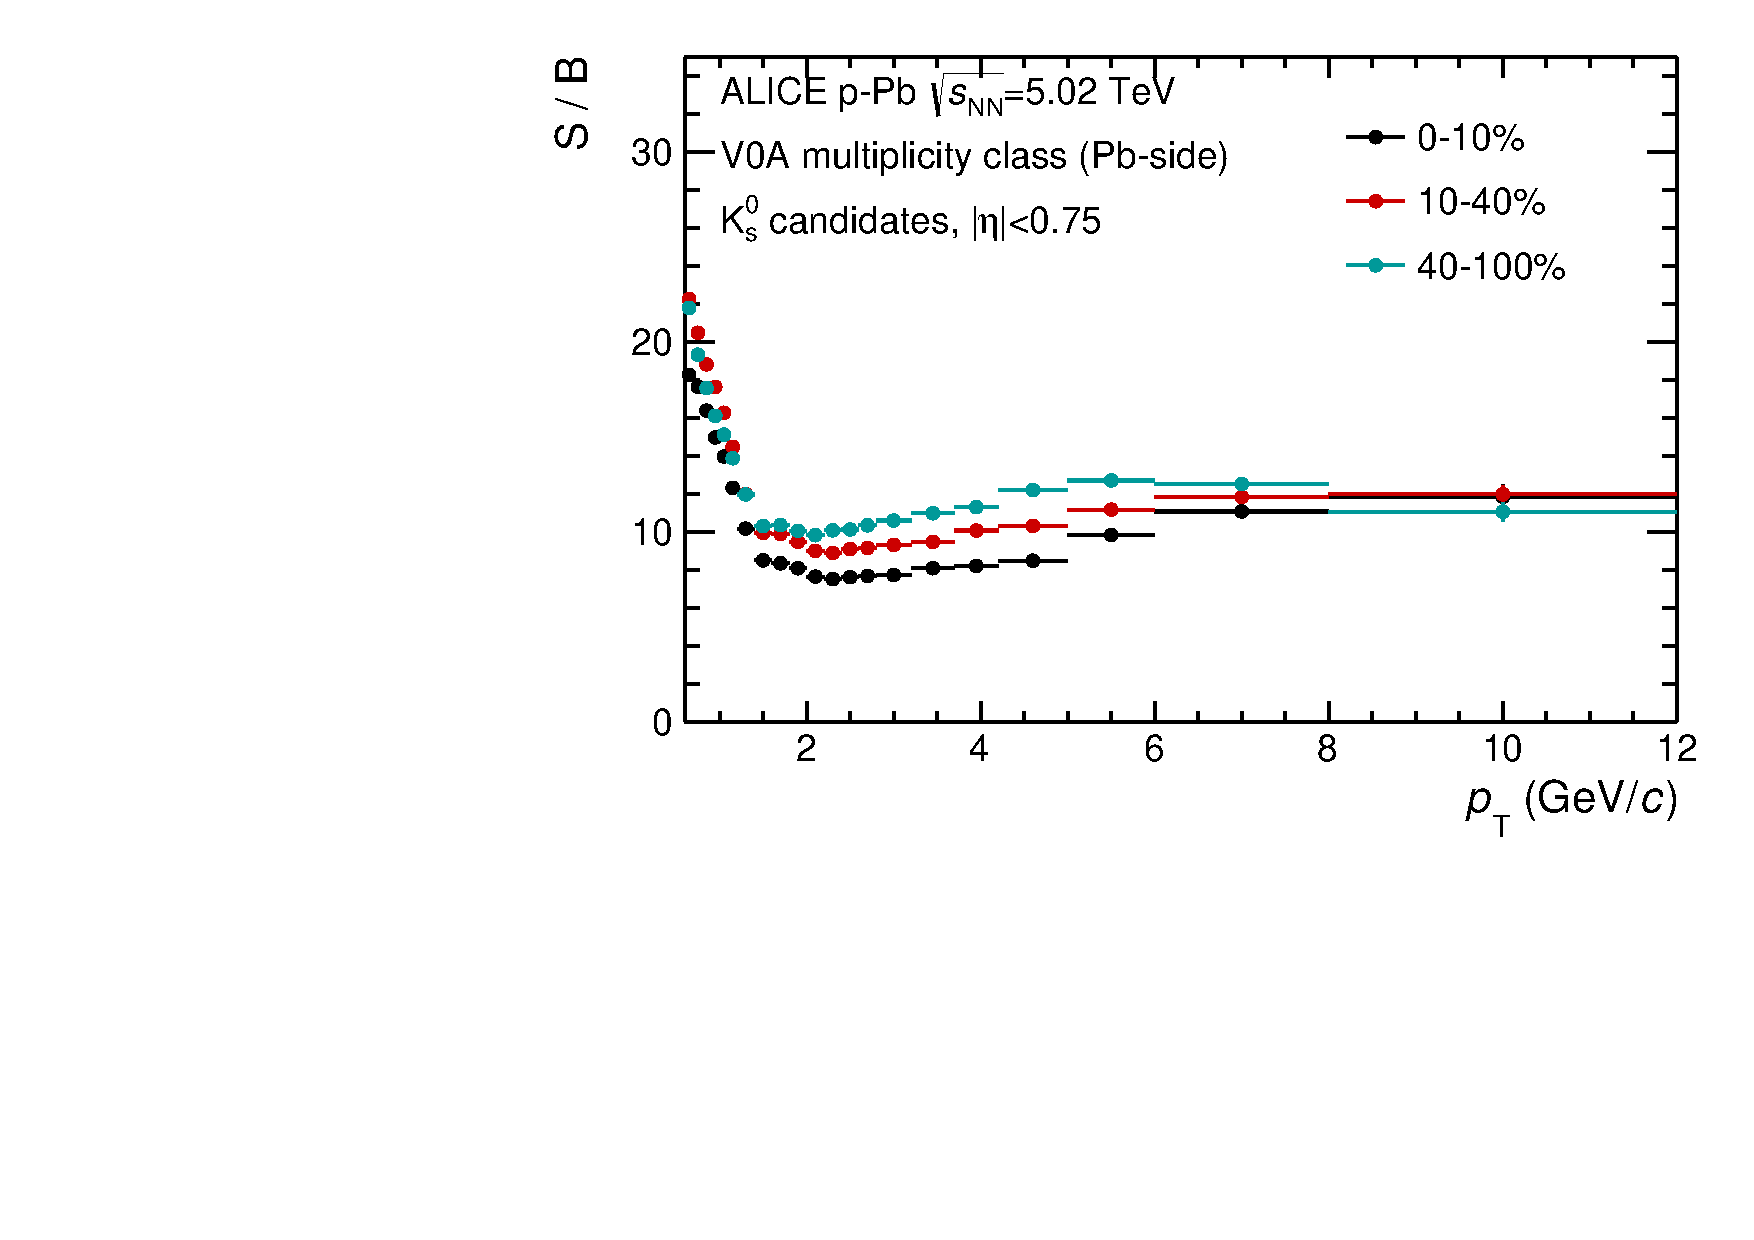
\includegraphics[width=.32\textwidth]{cS2Bratio_Kshort}
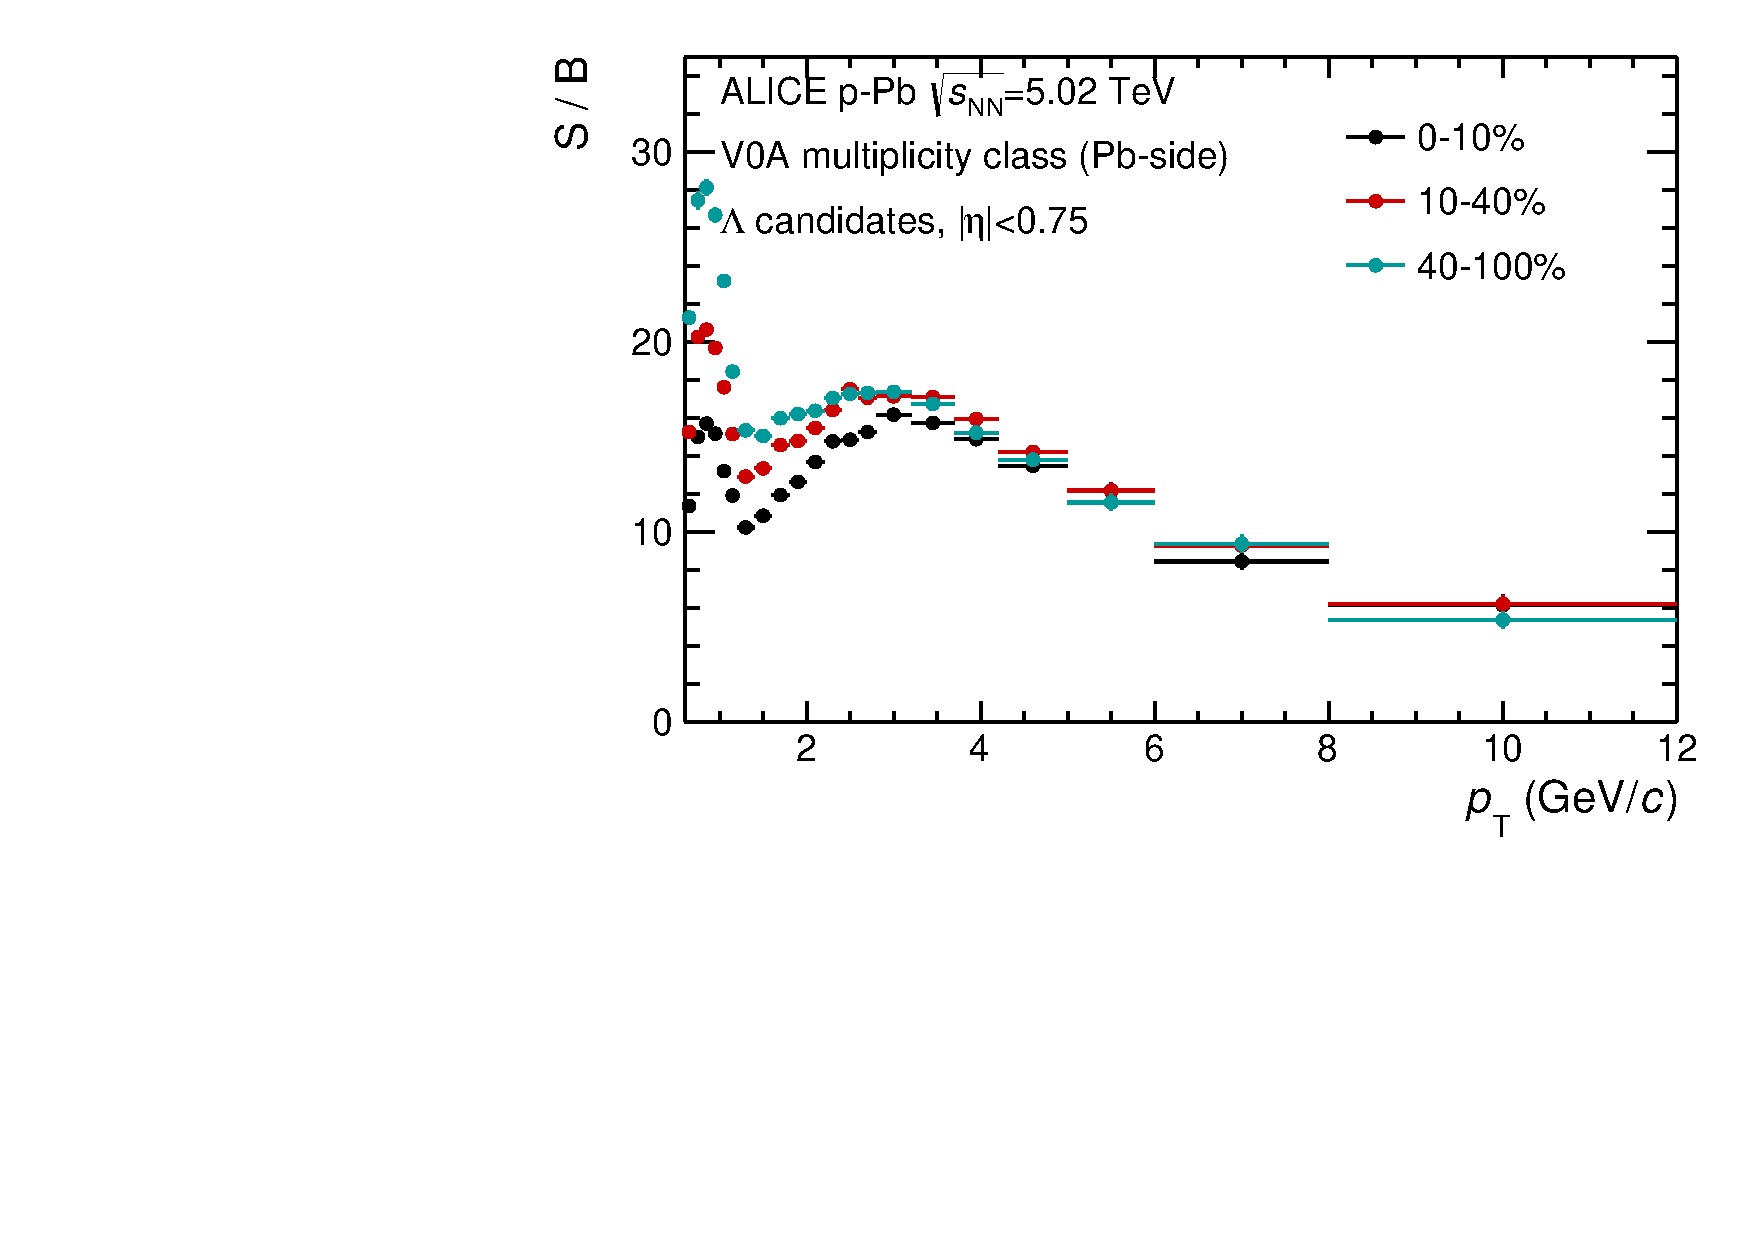
\includegraphics[width=.32\textwidth]{cS2Bratio_Lambda}
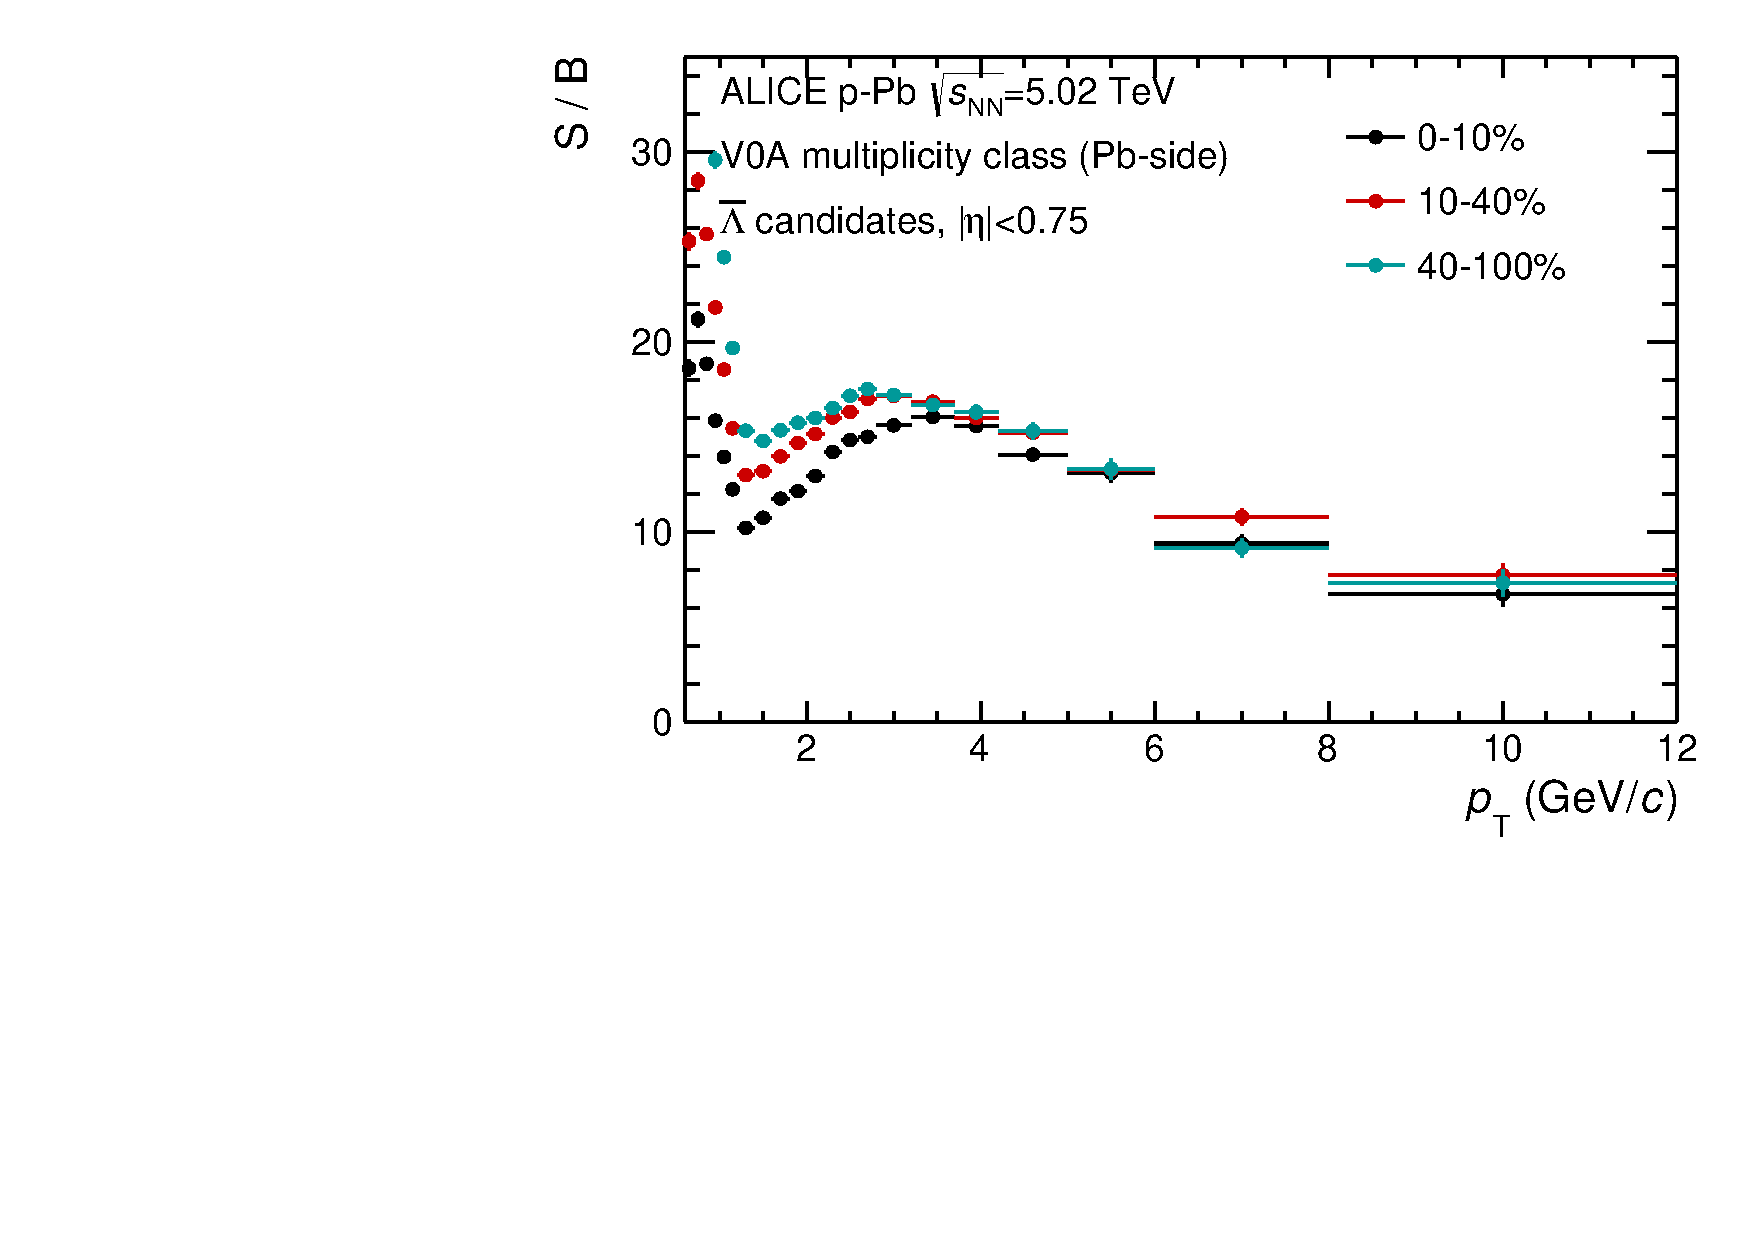
\includegraphics[width=.32\textwidth]{cS2Bratio_AntiLa}
\caption{S/B ratio of inclusive $\Vzero$s with default selection cuts.}
\label{fig:S2Bratio}
\end{figure}

Figure~\ref{fig:S2Bratio} shows the S/B ratio of inclusive $\Vzero$s with default selection cuts.
\conc{The S/B ratio is $\succsim 10$ and achieves to $20$ ($30$) for $\Kshort$ ($\Lambda$) at low $\pT$.} \\


\emplist{175}{5}{more details needed?}

\emp{To be added} \\


\emplist{185}{5}{check number}

I did not have a precise value of this fraction.
But a hint can be gotten from \emp{the figure in \textbf{p.~3} in~\cite{zhang:2013Jun}}.
It shows that the per-event multiplicity of jets in $\pT>10$~GeV/$c$ is $\mathcal{O}(10^{-3})$.
If the total number of MB events is $N$, then only $\sim 0.1\% N$ events contain the hard scattering which provides charged particle jets in $\pT>10$~GeV/$c$ (they may be di-jet events, but the away-side jet does not overlap to the nearside one).
With a simple estimation, the number of events which contain two (independent) tagged hard scatterings is $\sim(0.1\%)^{2}N$.
If the jet overlapping probability in such events is $\alpha~(<1)$, then the probability for a $\Vzero$ candidate match to two selected jets is
\begin{displaymath}
P\simeq\alpha(0.1\%)^{2}N/0.1\% N=\alpha 0.1\%<0.1\%.
\end{displaymath}
\conc{According to the above estimation, the number cited in the paper should be reasonable/safe.}

Indeed, the following approach was applied in the analysis to avoid double counting in the JC sample.
\begin{enumerate}
\item Loop over all $\Vzero$ candidates in a given event.
\item Tag the $\Vzero$ candidate as a JC $\Vzero$ if it can match to at least one selected jet.
\end{enumerate}
For calculating the JC $\Vzero$ acceptance (the area), the double counting of areas between two overlapped jets is avoided via a MC approach (see~\cite{zhang:1595alia} for details). \\


\emplist{225}{6}{MP: check numbers}

The feeddown fraction of inclusive $\Vzero$s and $\Vzero$s in jets are shown in \emp{figure~47 (p.~37) and figure~48 (p.~38) in~\cite{zhang:1595alia}}, respectively.
\conc{For  inclusive $\Vzero$s, the maximum feeddown correction is $<25\%$ and slightly depends on $\pT$, the feeddown correction of $\Vzero$s in jets is $\sim 15\%$ and is $\pT$ independent.} \\


\emplist{230}{8}{MP: remove the table; adjust the figure (remove fluctuations) and add the proper text}
\emplist{240}{8}{MP/Jana: Description in the figure does is not aligned with the description in the table. Uncertainties should be smoothed (local minima in some cases are unphysical).}

\emp{Working on the uncertainty flattening.} \\


\emplist{235}{7}{explain �competing $\Vzero$s� and �proper lifetime�}

Their definitions can be found in \emp{section~8 (p.~7) in~\cite{Ddobrigk:2012alia}}.
The cut values used in this analysis are listed in \emp{table~6 (p.~32) in~\cite{zhang:1595alia}}. \\


\emplist{240}{8}{Jana: Add explanation how the systematic uncertainties were propagated to the $\Lambda$/$\Kshort$ ratio.}
See \emp{section~\ref{sec:ratioErr} in this doc} for details. \\


\emplist{250}{8}{check numbers}

The values are returned in \emp{figure~3 in paper draft} and they are reasonable. \\


\emplist{260}{8}{check numbers}

The values are returned in \emp{figure~3 in paper draft}.
But the uncertainty on jet $\pT$ scale is slightly increasing with $\pT$ at high $\pT$ \emp{(to be discussed)}.
%%%%%%%%%%%%%%%%%%%%%%%%%%%%%%

\section{Efficiency}

\begin{figure}[t]
\centering
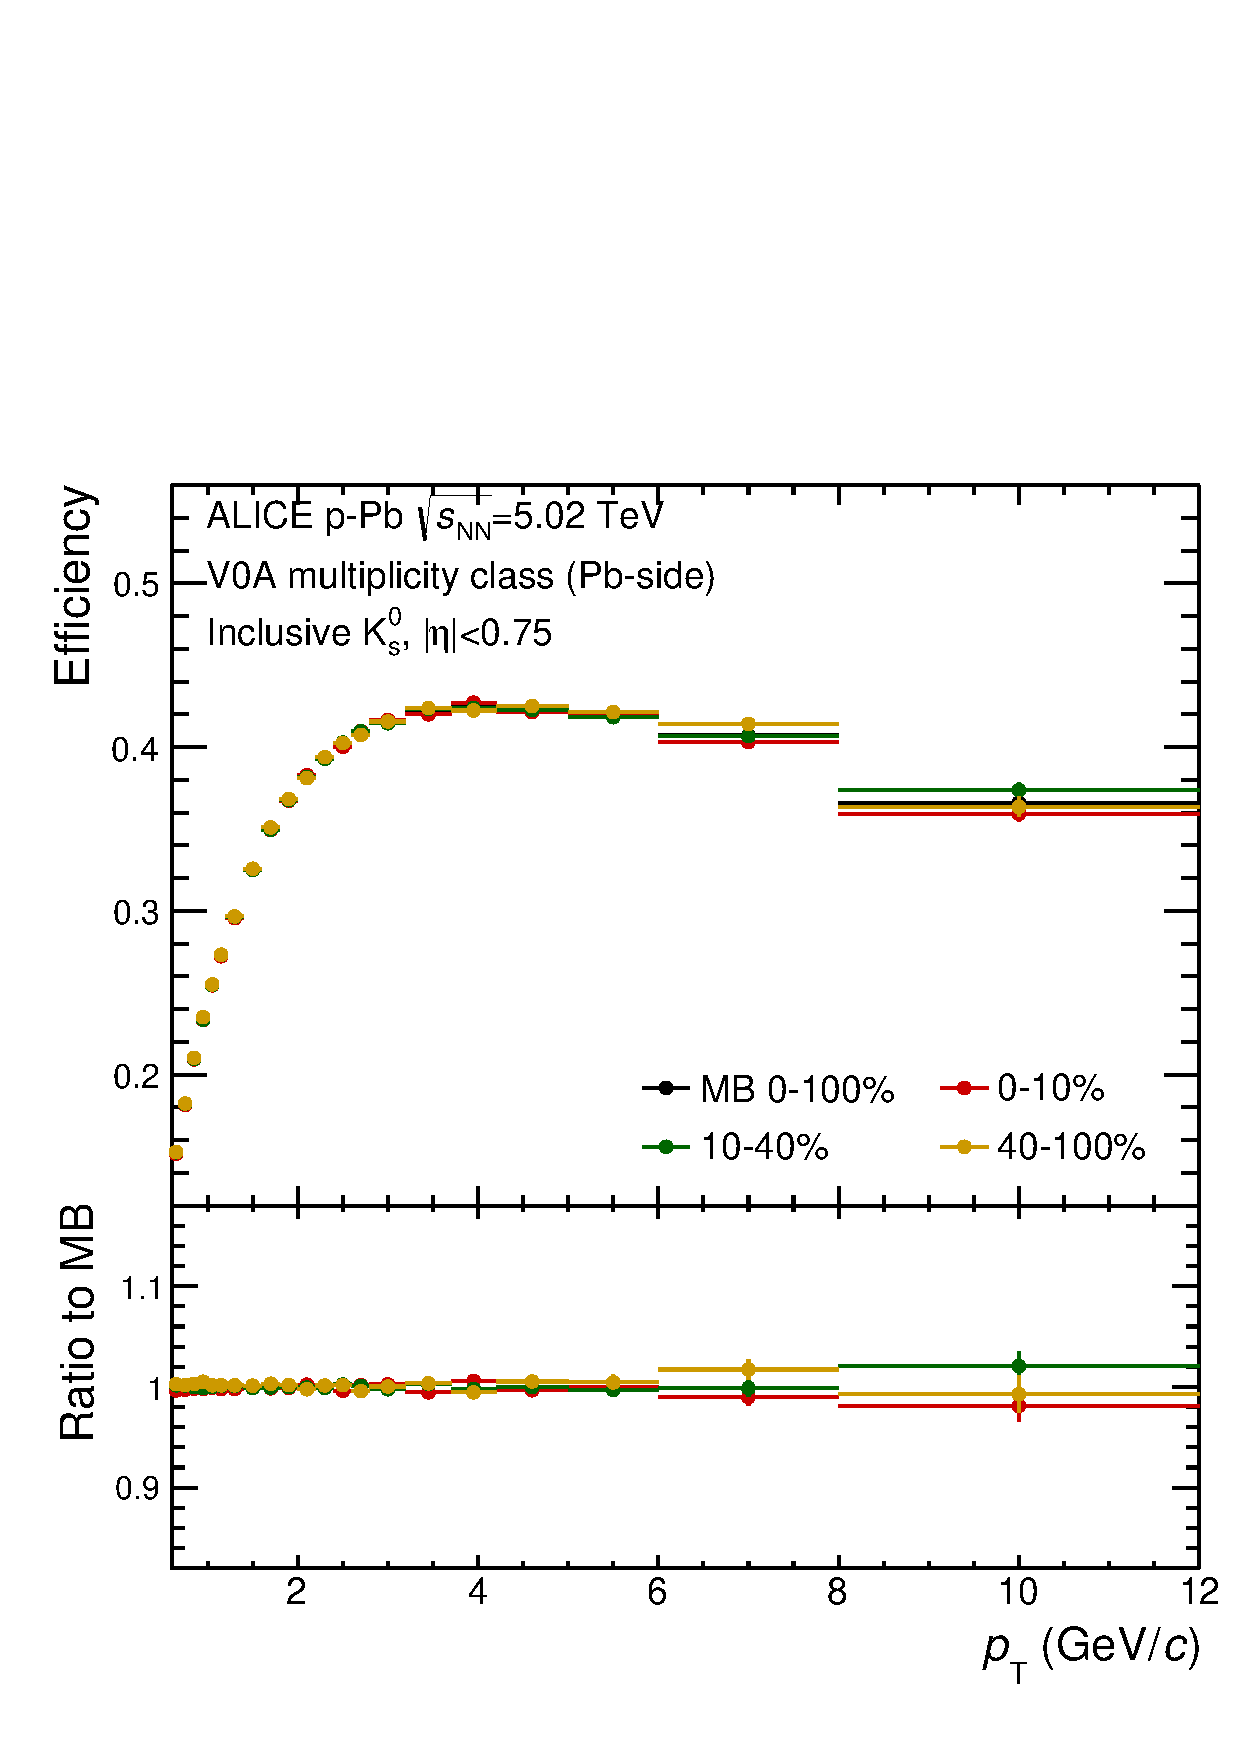
\includegraphics[width=.32\textwidth]{cEffiIncl_Kshort}
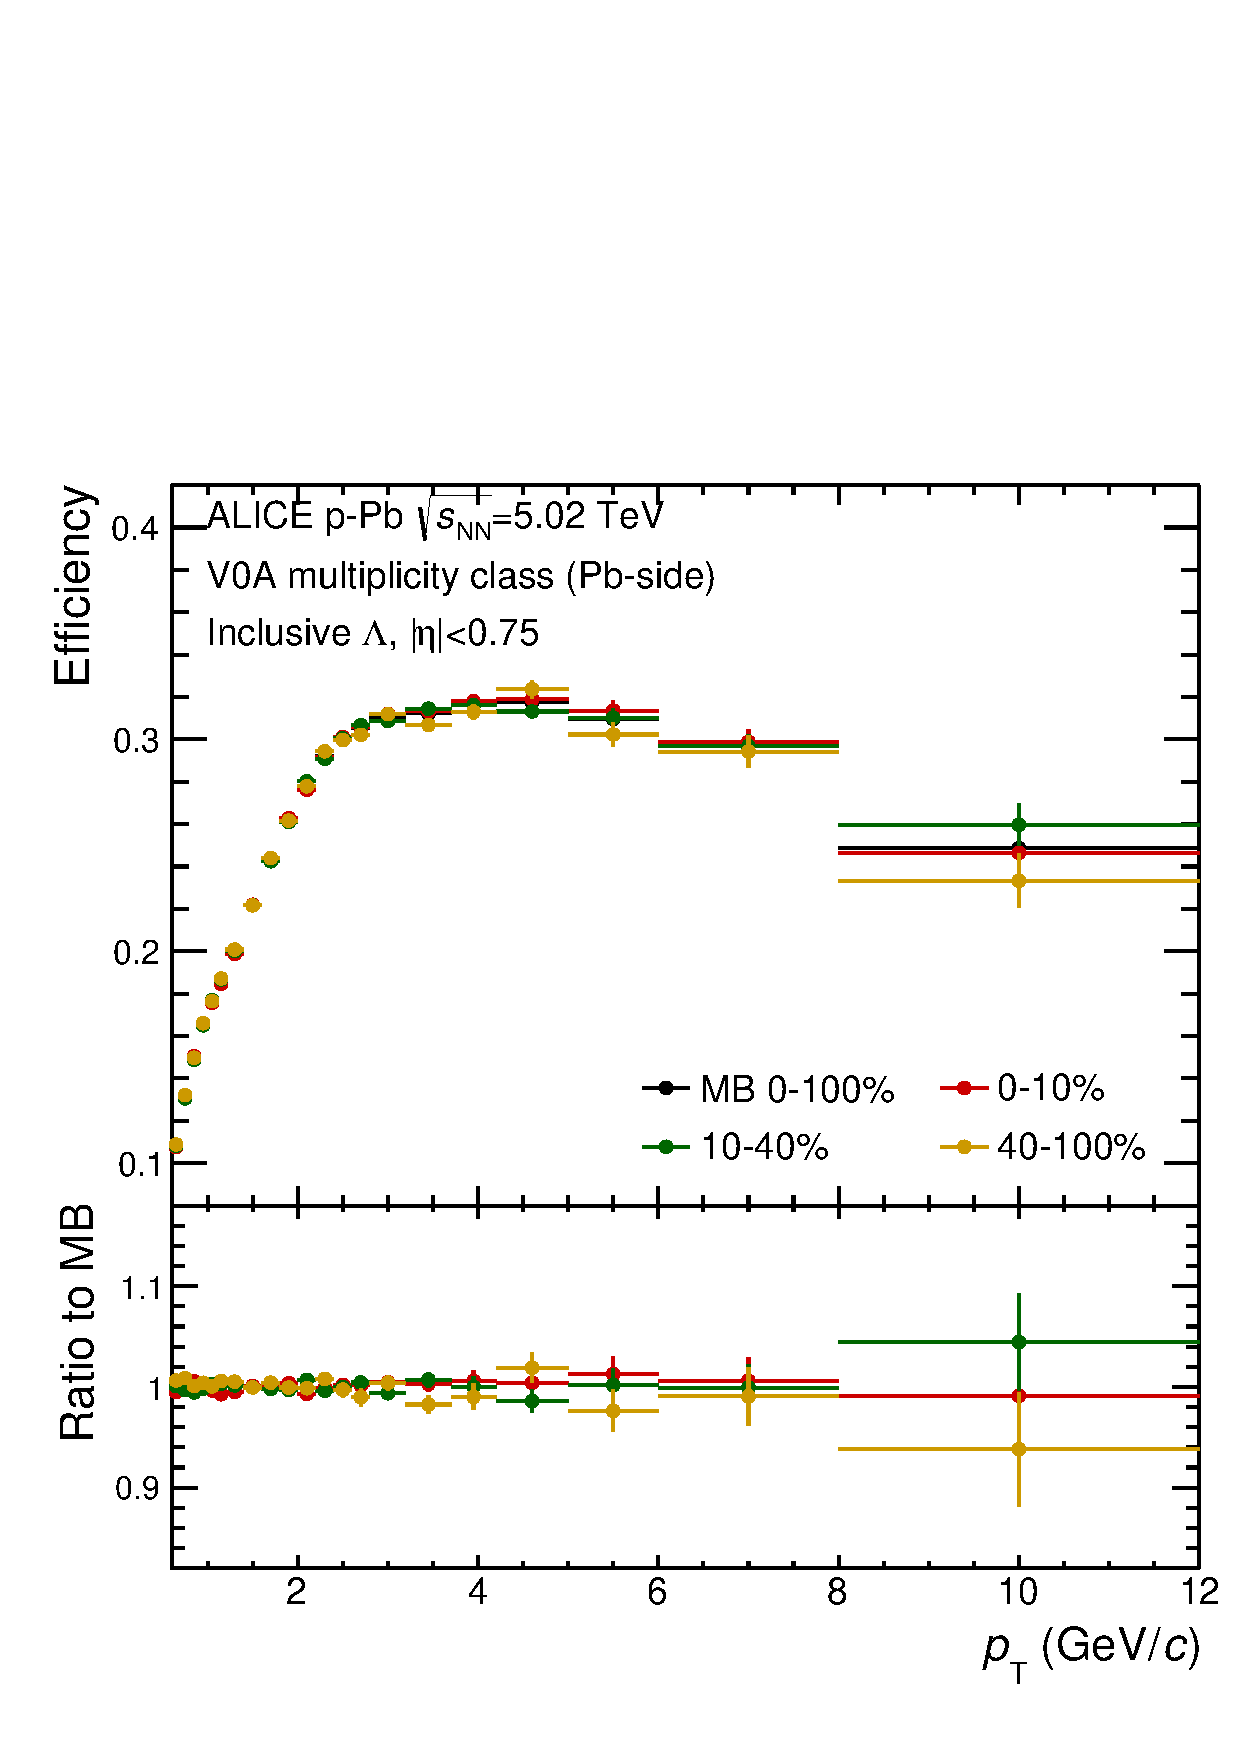
\includegraphics[width=.32\textwidth]{cEffiIncl_Lambda}
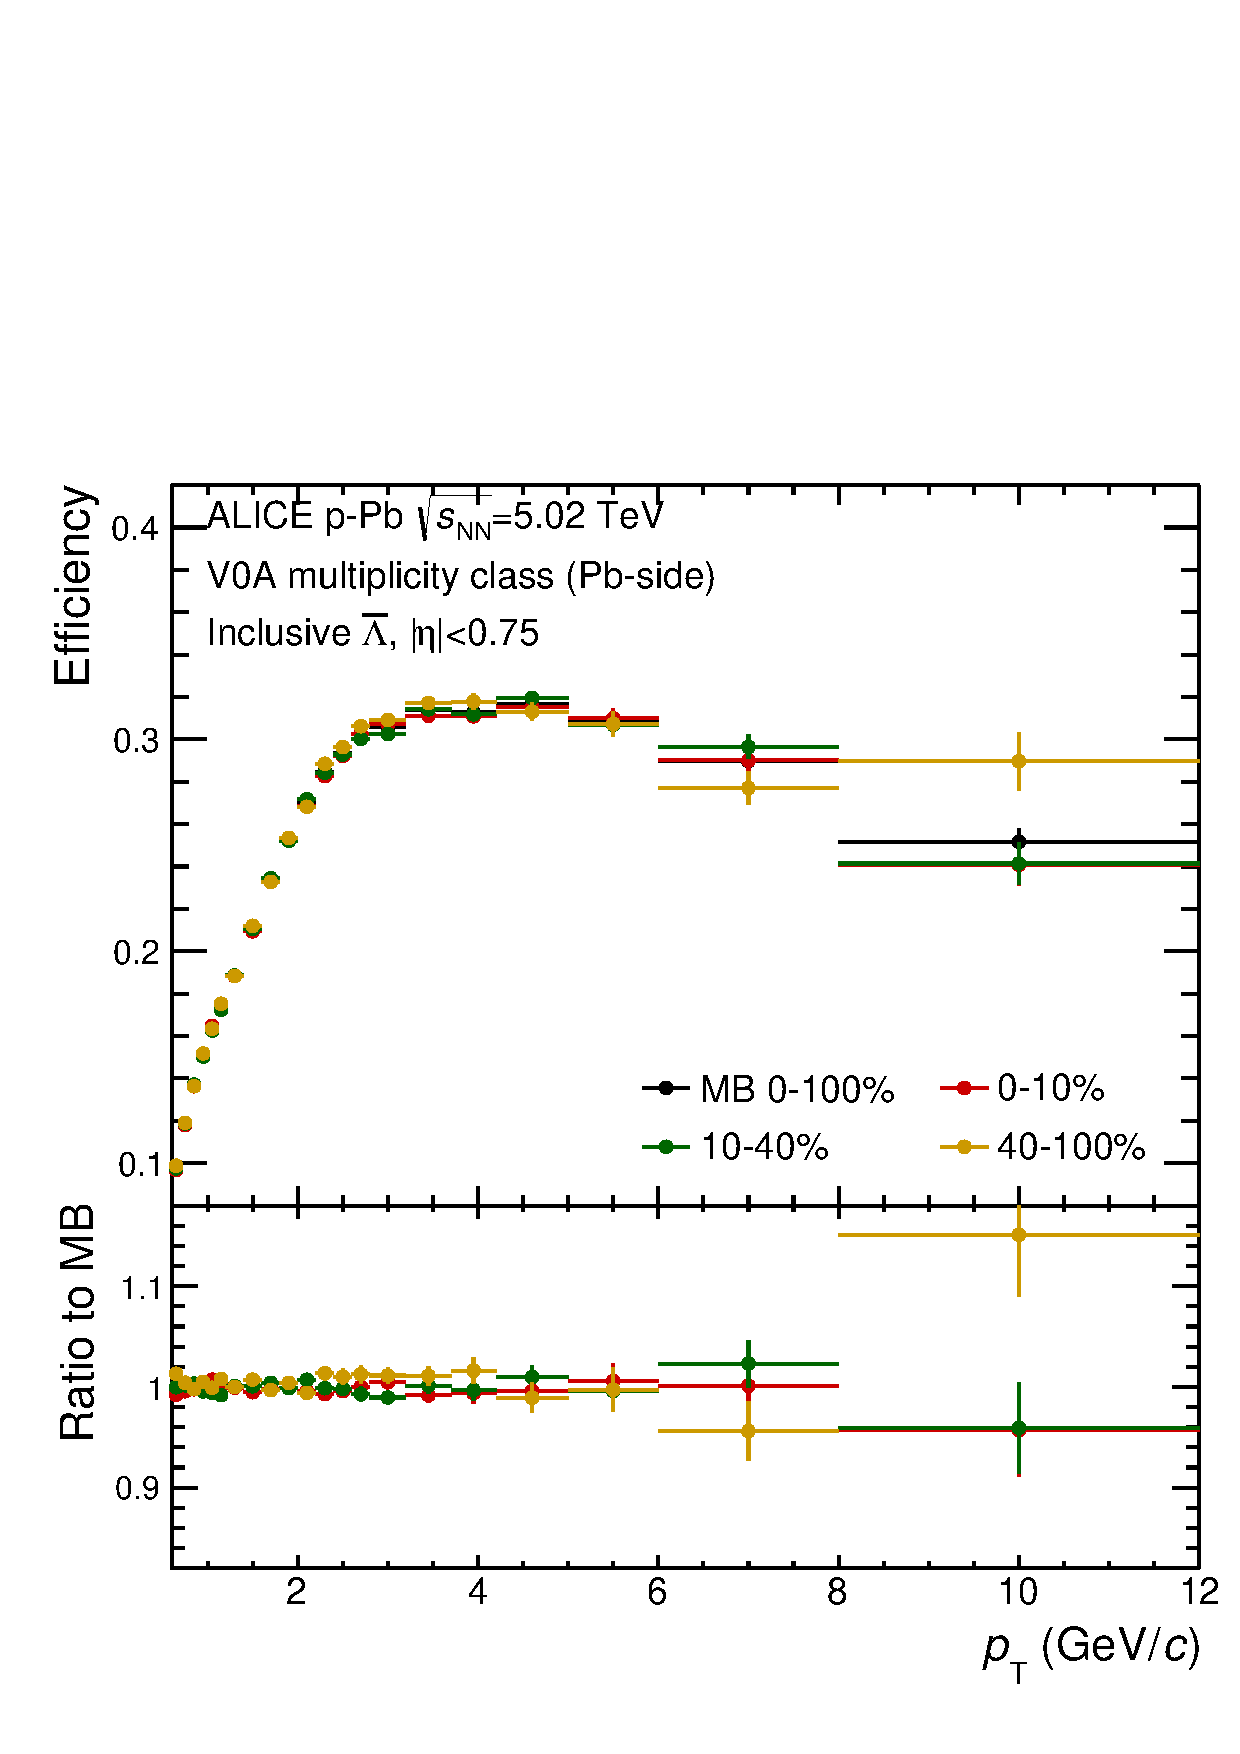
\includegraphics[width=.32\textwidth]{cEffiIncl_AntiLa}
\caption{Efficiency of inclusive $\Vzero$s in three event activities and MB events.}
\label{fig:EffiIncl}
\end{figure}

\begin{figure}[htbp]
\centering
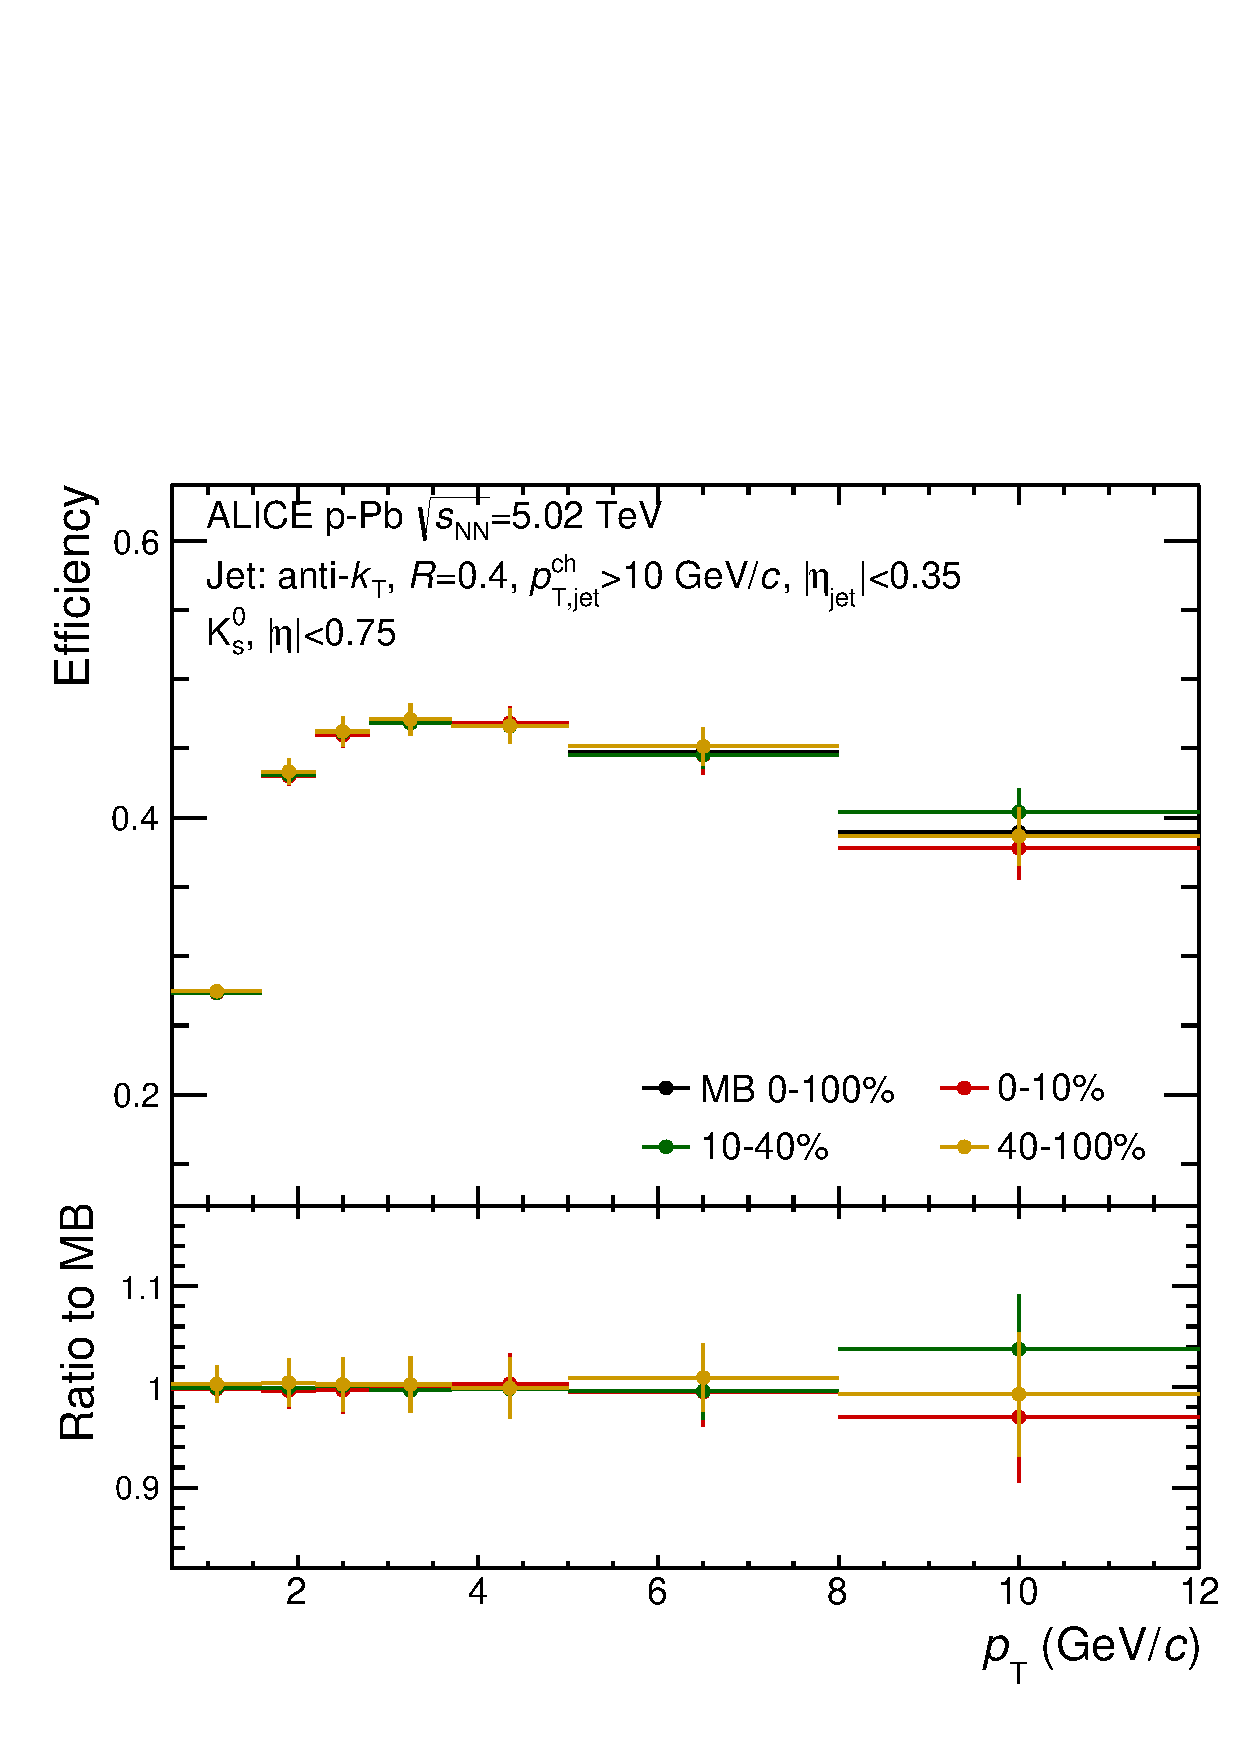
\includegraphics[width=.32\textwidth]{cEffi_KshortJC}
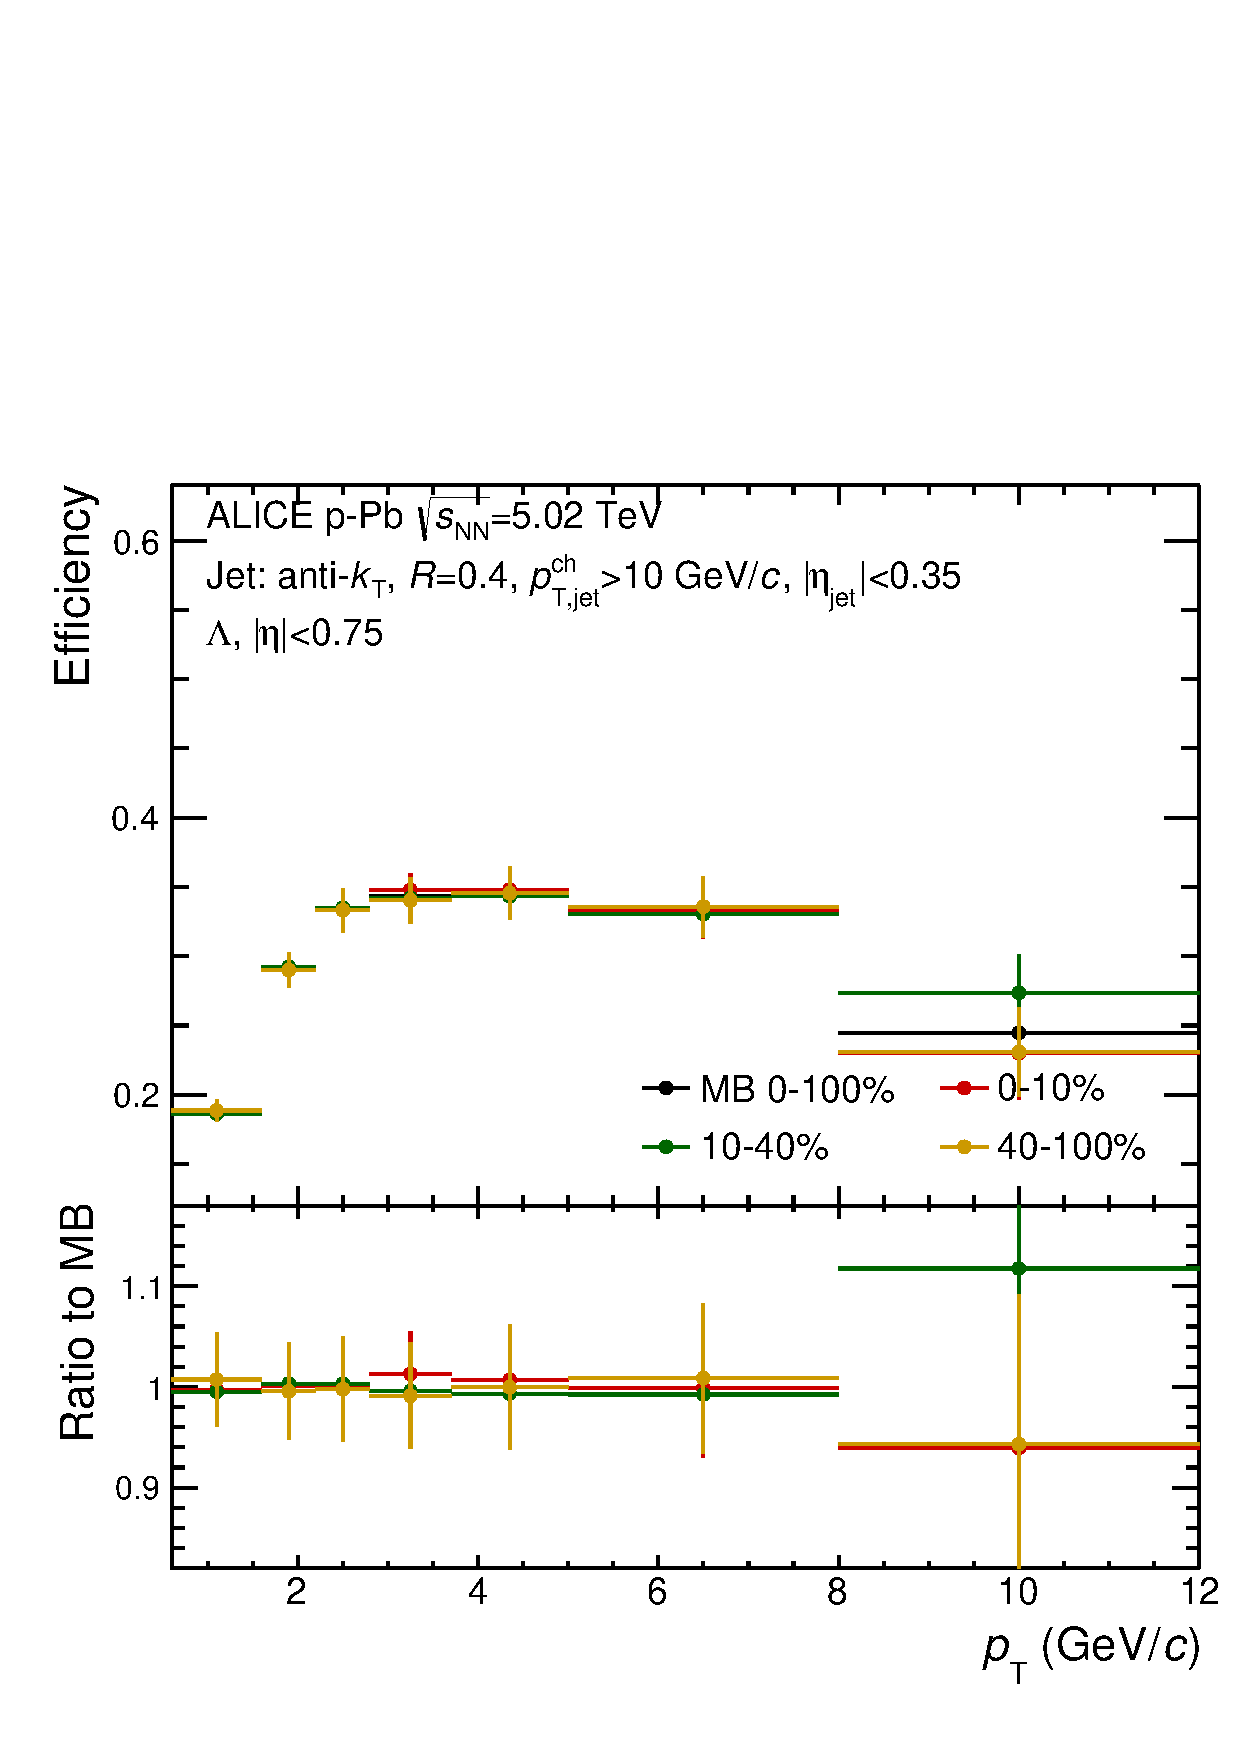
\includegraphics[width=.32\textwidth]{cEffi_LambdaJC}
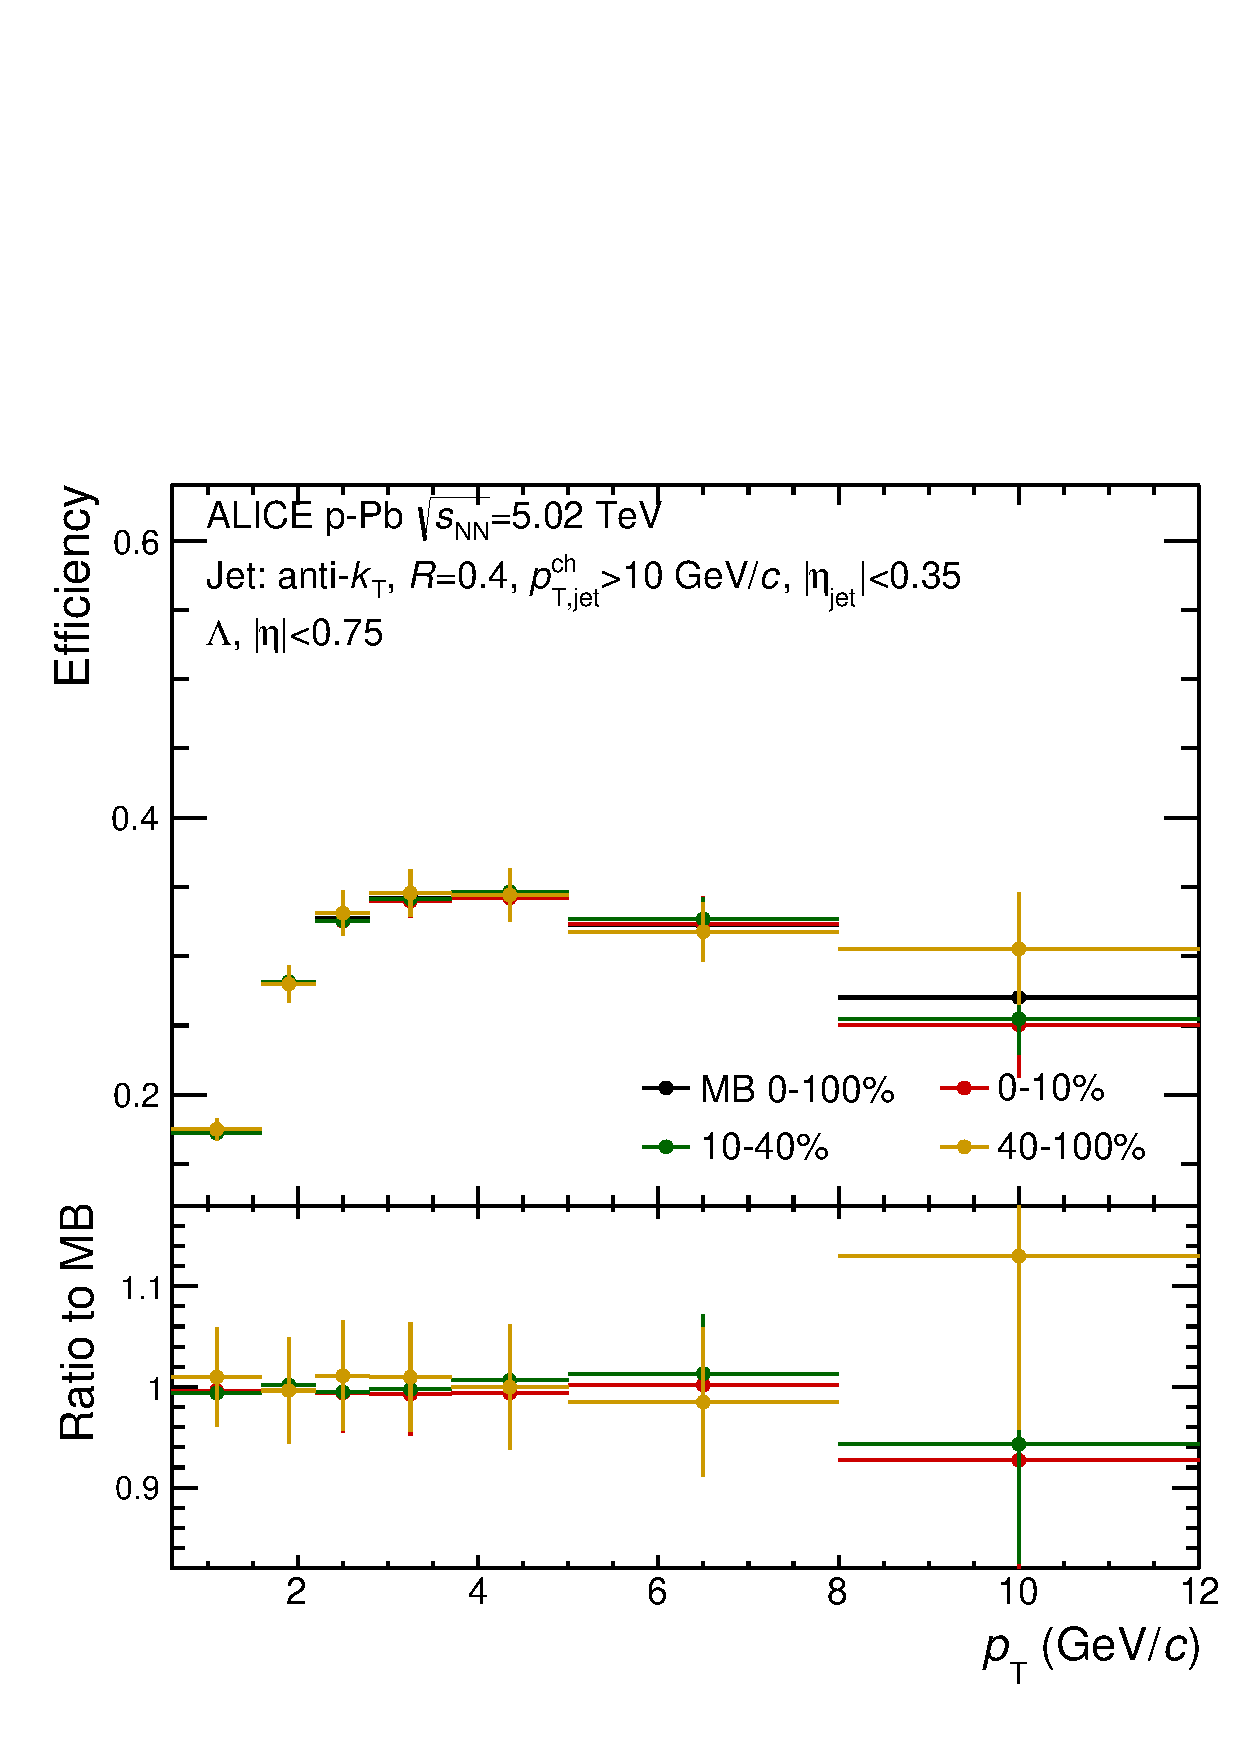
\includegraphics[width=.32\textwidth]{cEffi_AntiLaJC}
\caption{Efficiency of the $\Vzero$ in jets in three event activities and MB events.}
\label{fig:EffiJCV0s}
\end{figure}

The efficiency of inclusive $\Vzero$s and that of the $\Vzero$ in jets are shown in figure~\ref{fig:EffiIncl} and figure~\ref{fig:EffiJCV0s}, respectively.
The results are shown in three event activities and compared to that in MB events.
It shows that these two kind of efficiencies are insensitive to event multiplicity.

\emp{In paper, we used the efficiency in \cent{0}{10} event activity estimated by V0A.}
But these choice does not change any physics information, since:
\begin{itemize}
\item Efficiency is insensitive to event multiplicity.
\item Results in MB events should close to that \cent{0}{10} event activity due to the most central collisions have the largest (multiplicity) weight.
\end{itemize}

\conc{The efficiency in MB events will be used in the paper.}
%%%%%%%%%%%%%%%%%%%%%%%%%%%%%%

\section{Systematic uncertainty}

\subsection{\textcolor{blue}{Old uncertainty strategy for paper proposal}}

\subsubsection{Uncertainty source of inclusive $\Vzero$s}

The source of systematic uncertainty of inclusive $\Vzero$s is concluded in~\cite{zhang:1595alia} see also~\cite{Ddobrigk:2012alia} for details. It includes:
\begin{itemize}
\item Uncertainty on $\Vzero$ yields
\item Uncertainty on material budget
\item Uncertainty on feeddown correction (for $\Lambda$ and $\AntiLa$)
\end{itemize}
The first one is obtained in this analysis and the other two are taken from~\cite{Abelev:2013haa} since these two analyses used the same data and MC samples. The uncertainty on $\Vzero$ yields contains:
\begin{enumerate}
\item Topological selections
\item Proper lifetime selection
\item Competing $\Vzero$ rejection
\item Track selection in TPC
\item Track PID in TPC
\item Signal extraction
\end{enumerate}
in which
\begin{itemize}
\item The uncertainty on \emp{topological selections} is obtained by varying five kind of cuts defined in \emp{table~5 (p.~32) in~\cite{zhang:1595alia}}, results are shown in \emp{figure~42 (p.~33) in~\cite{zhang:1595alia}}.
\item The uncertainty on \emp{track selection in TPC} is dependent on two variables defined in \emp{table~7 (p.~32) in~\cite{zhang:1595alia}}, results are shown in \emp{figure~43 (p.~34)in~\cite{zhang:1595alia}}.
\item \emp{Other uncertainties on $\Vzero$ yields} are obtained by following the same \emp{criteria defined in~\cite{Ddobrigk:2012alia}}.
\end{itemize}
The sources of systematic uncertainty on $\Vzero$ yields are shown in figure~\ref{fig:SystIncl}.

\begin{figure}[t]
\centering
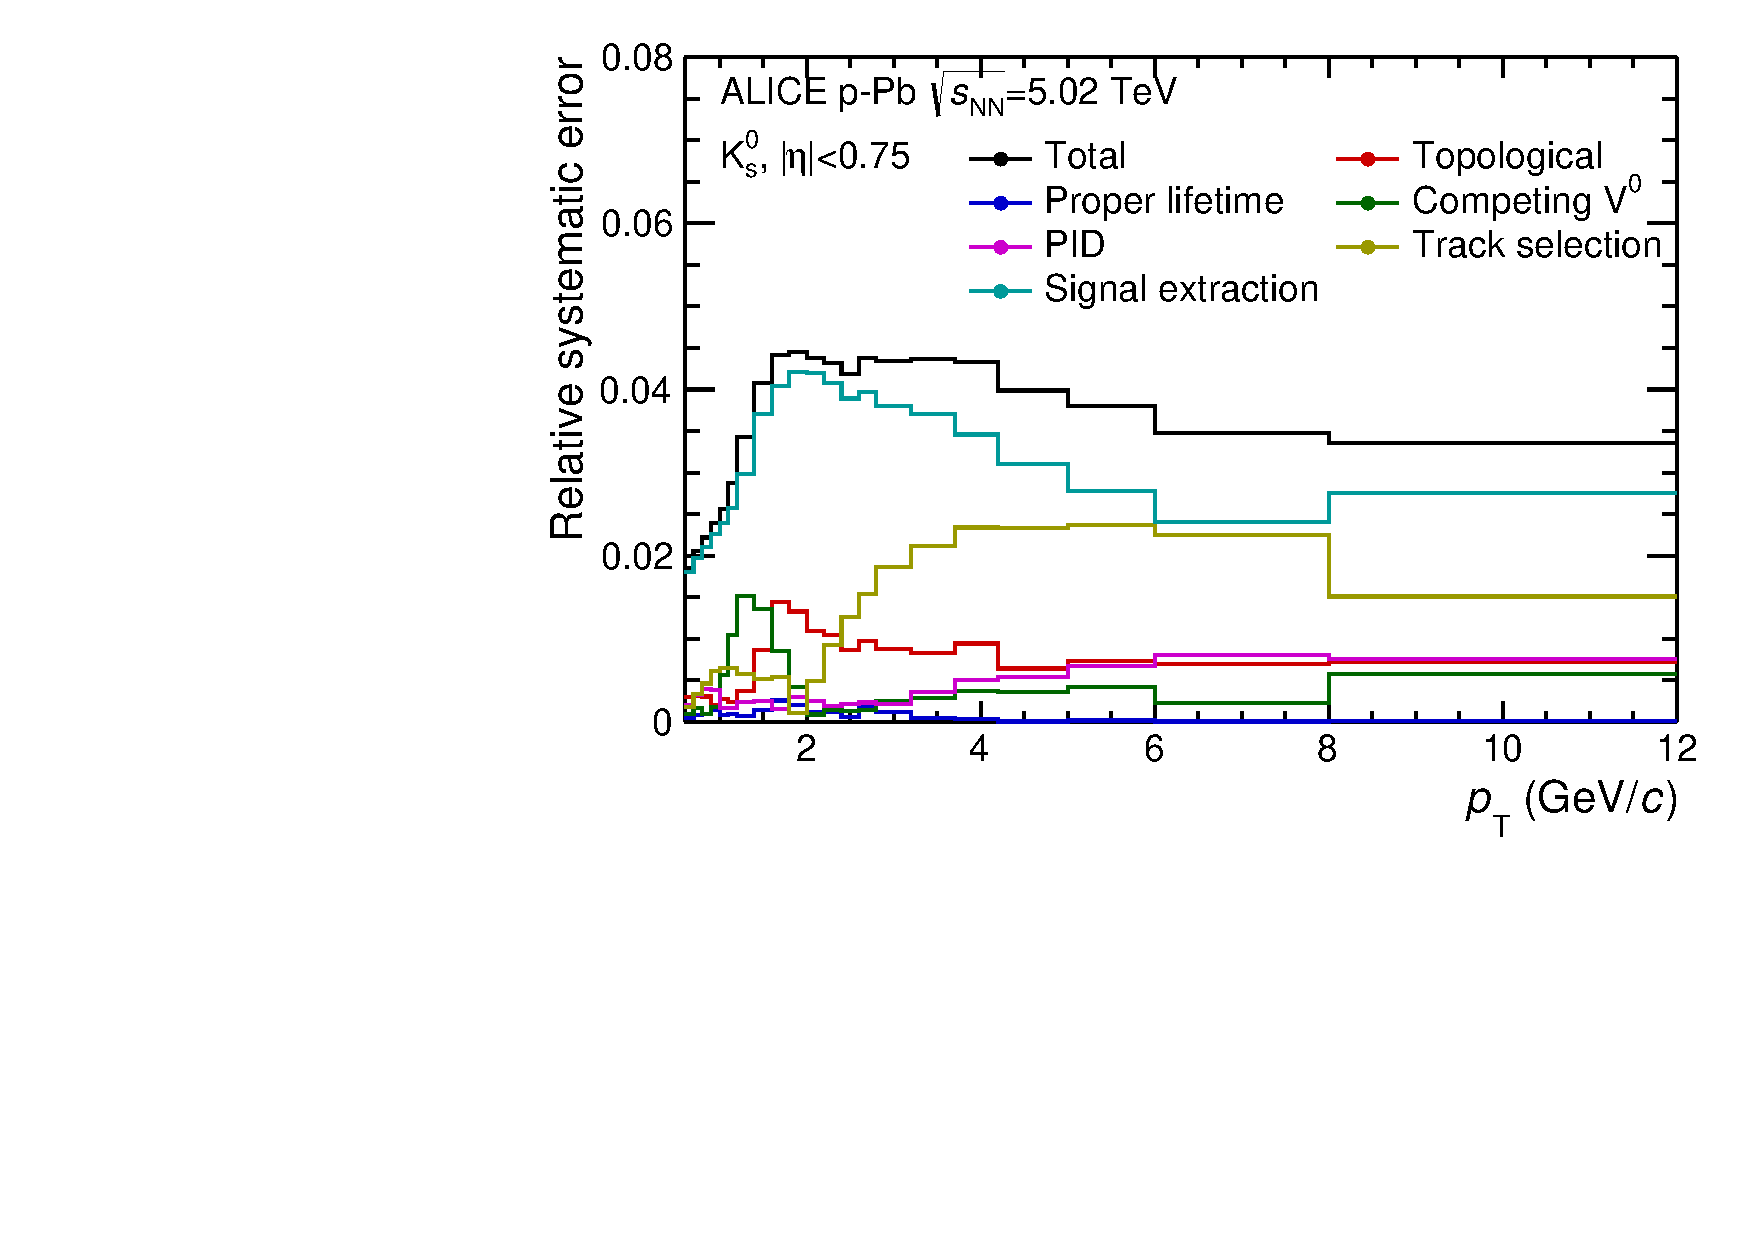
\includegraphics[width=.32\textwidth]{cSystIncl_Kshort}
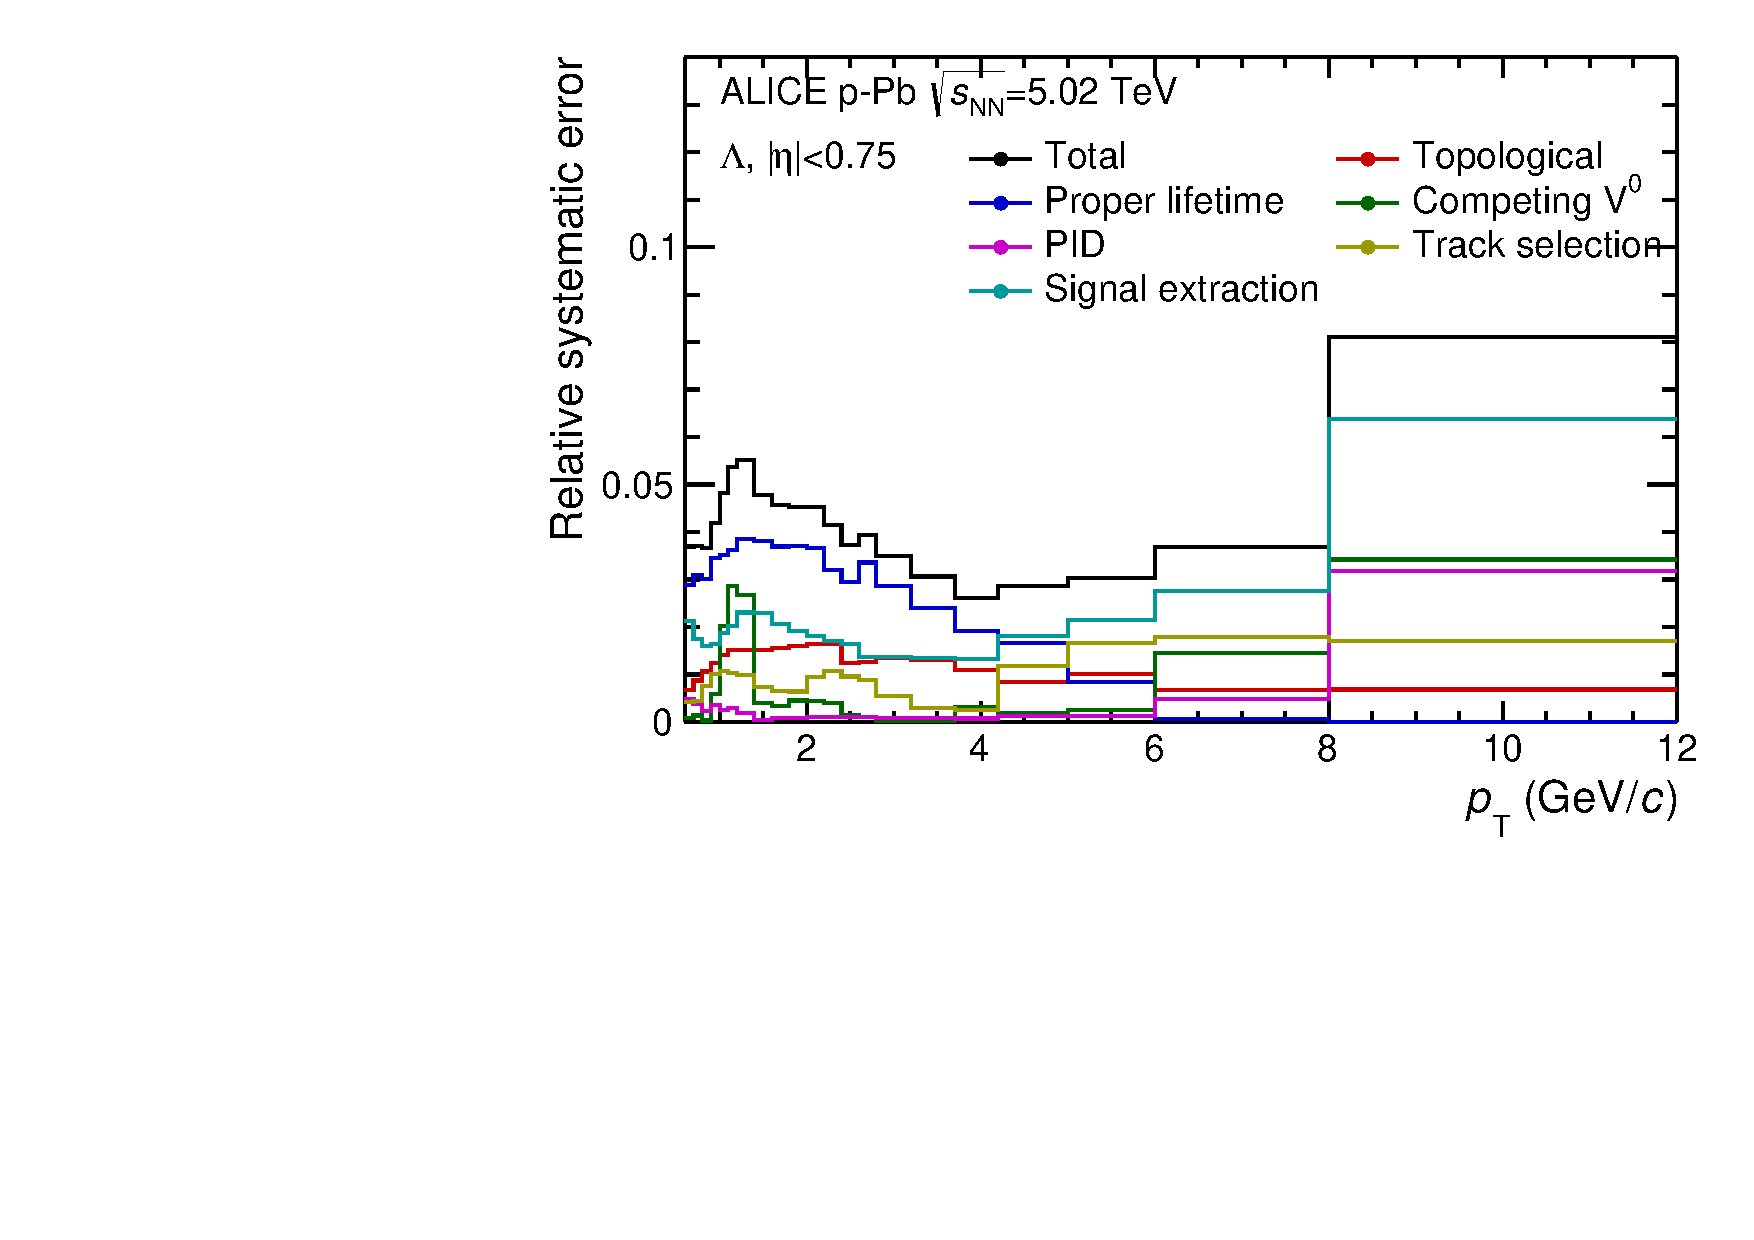
\includegraphics[width=.32\textwidth]{cSystIncl_Lambda}
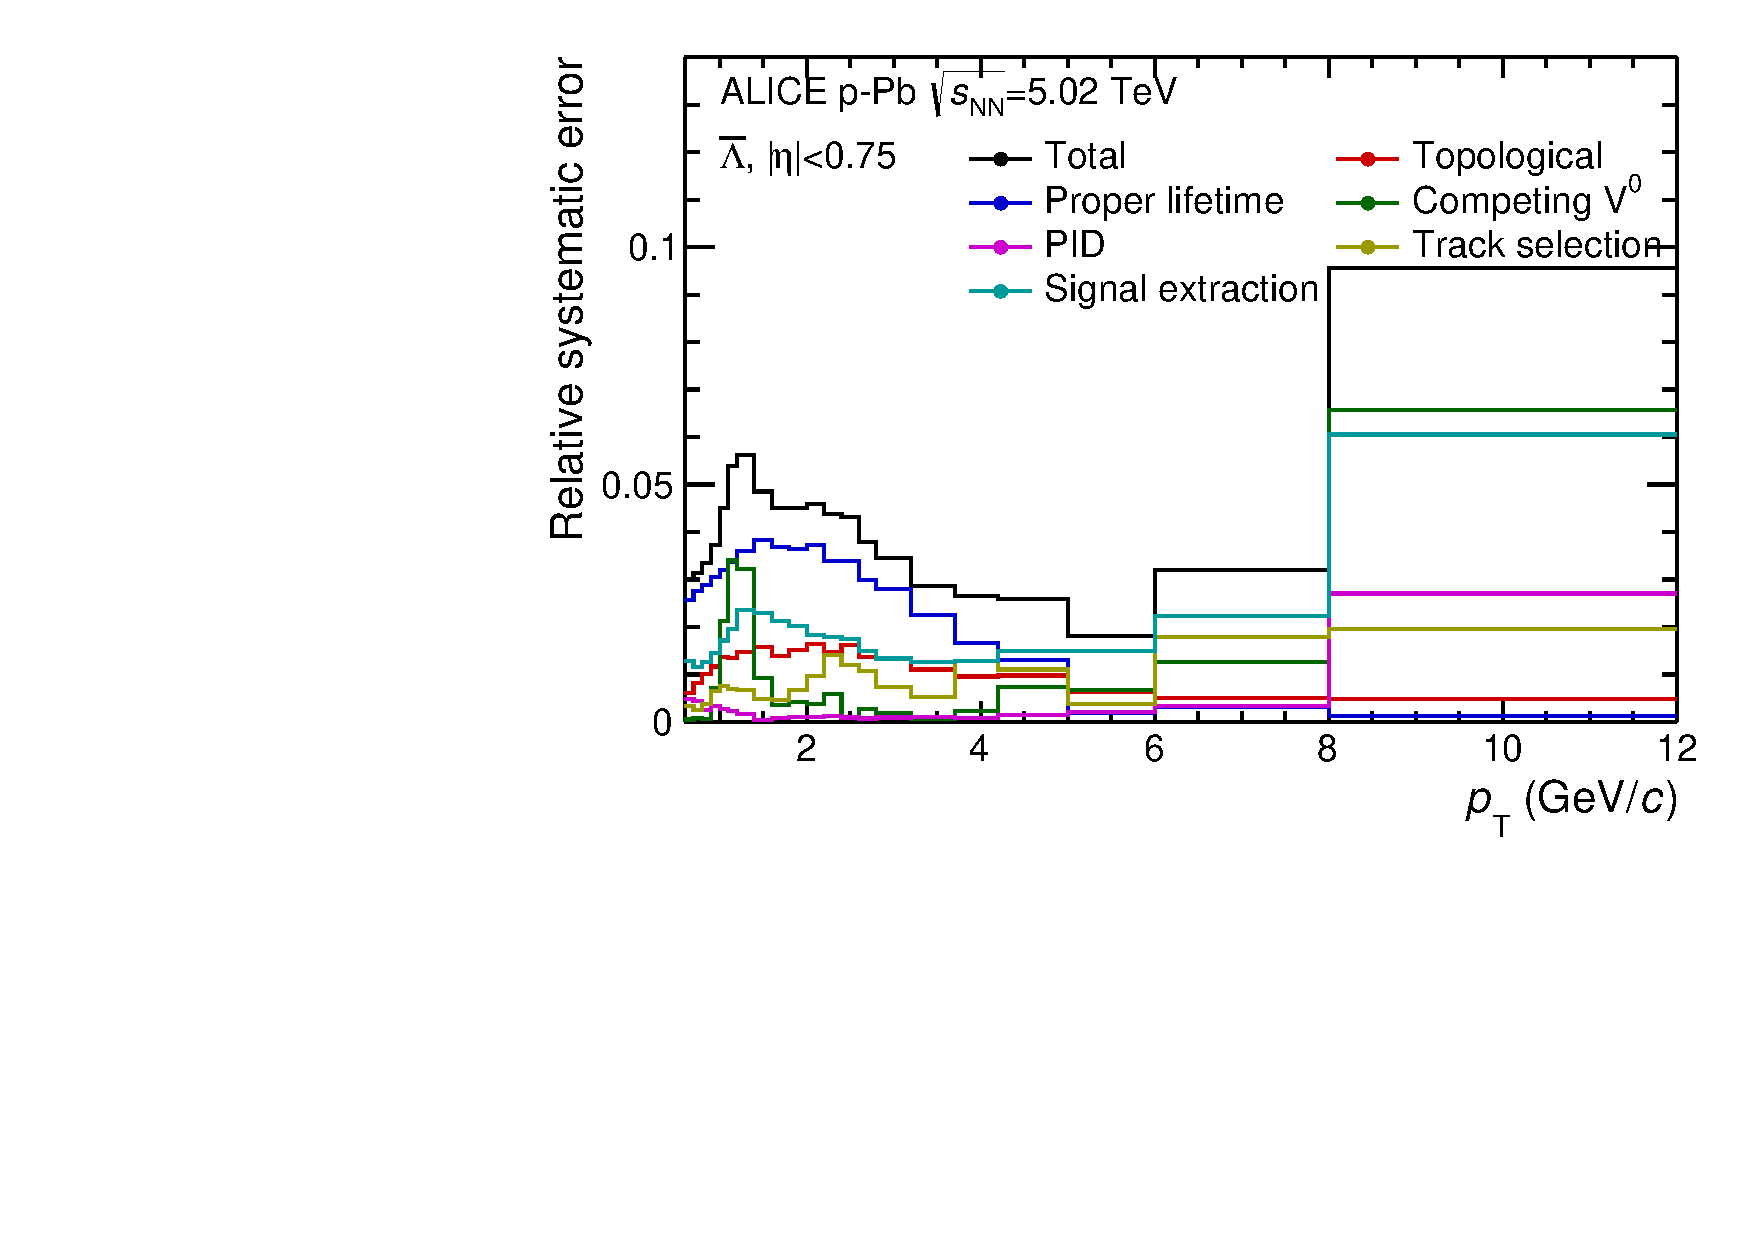
\includegraphics[width=.32\textwidth]{cSystIncl_AntiLa}
\caption{Systematic uncertainty of inclusive $\Vzero$s.}
\label{fig:SystIncl}
\end{figure}

\subsubsection{Systematic uncertainty of $\Vzero$s in jets}

The uncertainty source of $\Vzero$s in jets includes:
\begin{itemize}
\item Uncertainty on $\Vzero$ yields
\item Uncertainty on material budget
\item Uncertainty on feeddown correction
\item Uncertainty on jet $\pT$ scale
\item Uncertainty on UE estimation
\end{itemize}
in which the \emp{uncertainty on material budget} is taken from~\cite{Abelev:2013haa} and the same as inclusive $\Vzero$s. \\

For $\Vzero$s in jets, the \emp{uncertainty on $\Vzero$ yields} has the same sources as inclusive $\Vzero$s. But they are separated into two catalogs:
\begin{itemize}
\item Uncertainty independent on statistics (the first five uncertainty sources)
\item Uncertainty depend on statistics (the last one \emp{uncertainty on signal extraction})
\end{itemize}
The uncertainties in the first catalog is taken from the inclusive analysis directly.
The last uncertainty is estimated by using $\Vzero$s matched to the jet with the same criteria as inclusive $\Vzero$s. The \emp{uncertainty on signal extraction} is sensitive to statistic fluctuations \emp{a constant value of $6\%$ ($10\%$) is aligned to $\Vzero$s in jets in $\pT>10$~GeV/$c$ ($>20$~GeV/$c$)}. \\

By considering the feeddown contribution for inclusive $\Vzero$s and $\Vzero$s in jets may be different, based on \textsc{PYTHIA} simulations, \emp{an additional $5\%$ uncertainty is added in uncertainty on feeddown correction} to cover the difference. \\

\emp{Uncertainty on jet $\pT$ scale} is estimated by varying the jet $\pT$ within $20\%$: \emp{$2$~GeV/$c$ ($4$~GeV/$c$) for $p_{\rm T,jet}=10$~GeV/$c$ ($20$~GeV/$c$)}. \\

\emp{Uncertainty on UE estimation} is obtained via different estimators. The default value is given by PC estimator. The uncertainty is estimated via the OC and NJ estimators.

\subsubsection{Uncertainty propagation}\label{sec:ratioErr}

The uncertainty of $\Lambda$/$\Kshort$ ratio is obtained via the following approach:
\begin{enumerate}
\item The uncertainties on $\Vzero$ yields, material budget and feeddown correction are propagated to the ratio quadratically (the standard way). \emp{Note: according to ref~\cite{Ddobrigk:2012alia} and \cite{Abelev:2013haa} the uncertainty on material budget should NOT been cancelled in the ratio.}
\item For the uncertainties on jet $\pT$ scale and UE estimation, they are obtained by calculating the deviation of ratios between the default  value and various selections.
\end{enumerate}

\subsection{\textcolor{red}{Improved uncertainty strategy}}

\begin{itemize}
\item For inclusive $\Vzero$s, flattening uncertainty on signal extraction at high $\pT$.
The observed increasing trend at high $\pT$ is (partly) due to the statistic fluctuations.
A flattening procedure is applied for overcoming the high-$\pT$ fluctuations.
Figure~\ref{fig:NewInclSyst} shows the updated uncertainty on $\Vzero$ yield of inclusive $\Vzero$s.
The uncertainty curves are smoothed to overcome local fluctuations.
\item For $\Vzero$s in jets, uncertainty on $\Vzero$ yields, now, is fully taken from that of inclusive $\Vzero$s.
There is no physics reason shows that this uncertainty should be different between $\Vzero$s in jets and inclusive $\Vzero$s.
Using the uncertainty of inclusive $\Vzero$s avoids statistic fluctuations.
\end{itemize}

\begin{figure}[t]
\centering
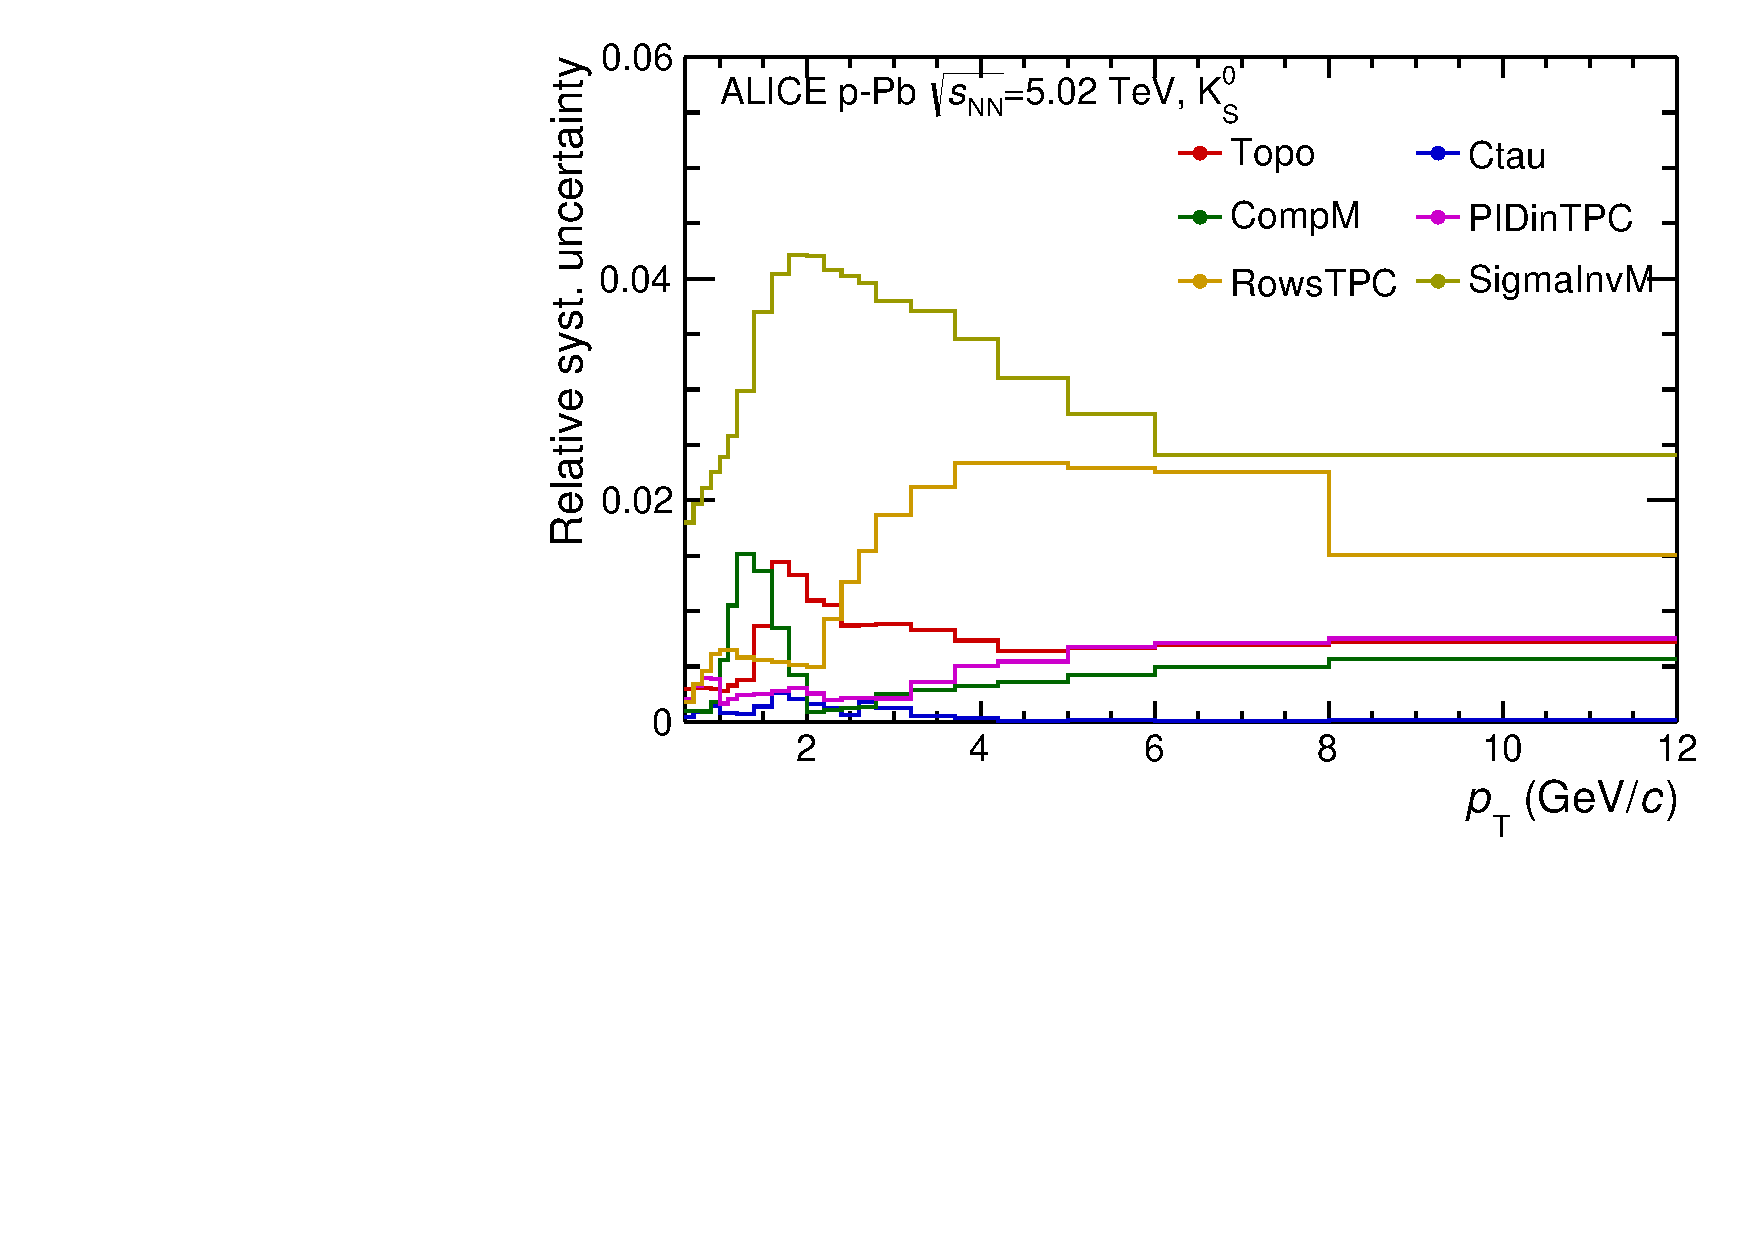
\includegraphics[width=.32\textwidth]{cCheckIncl_Kshort_Bin21}
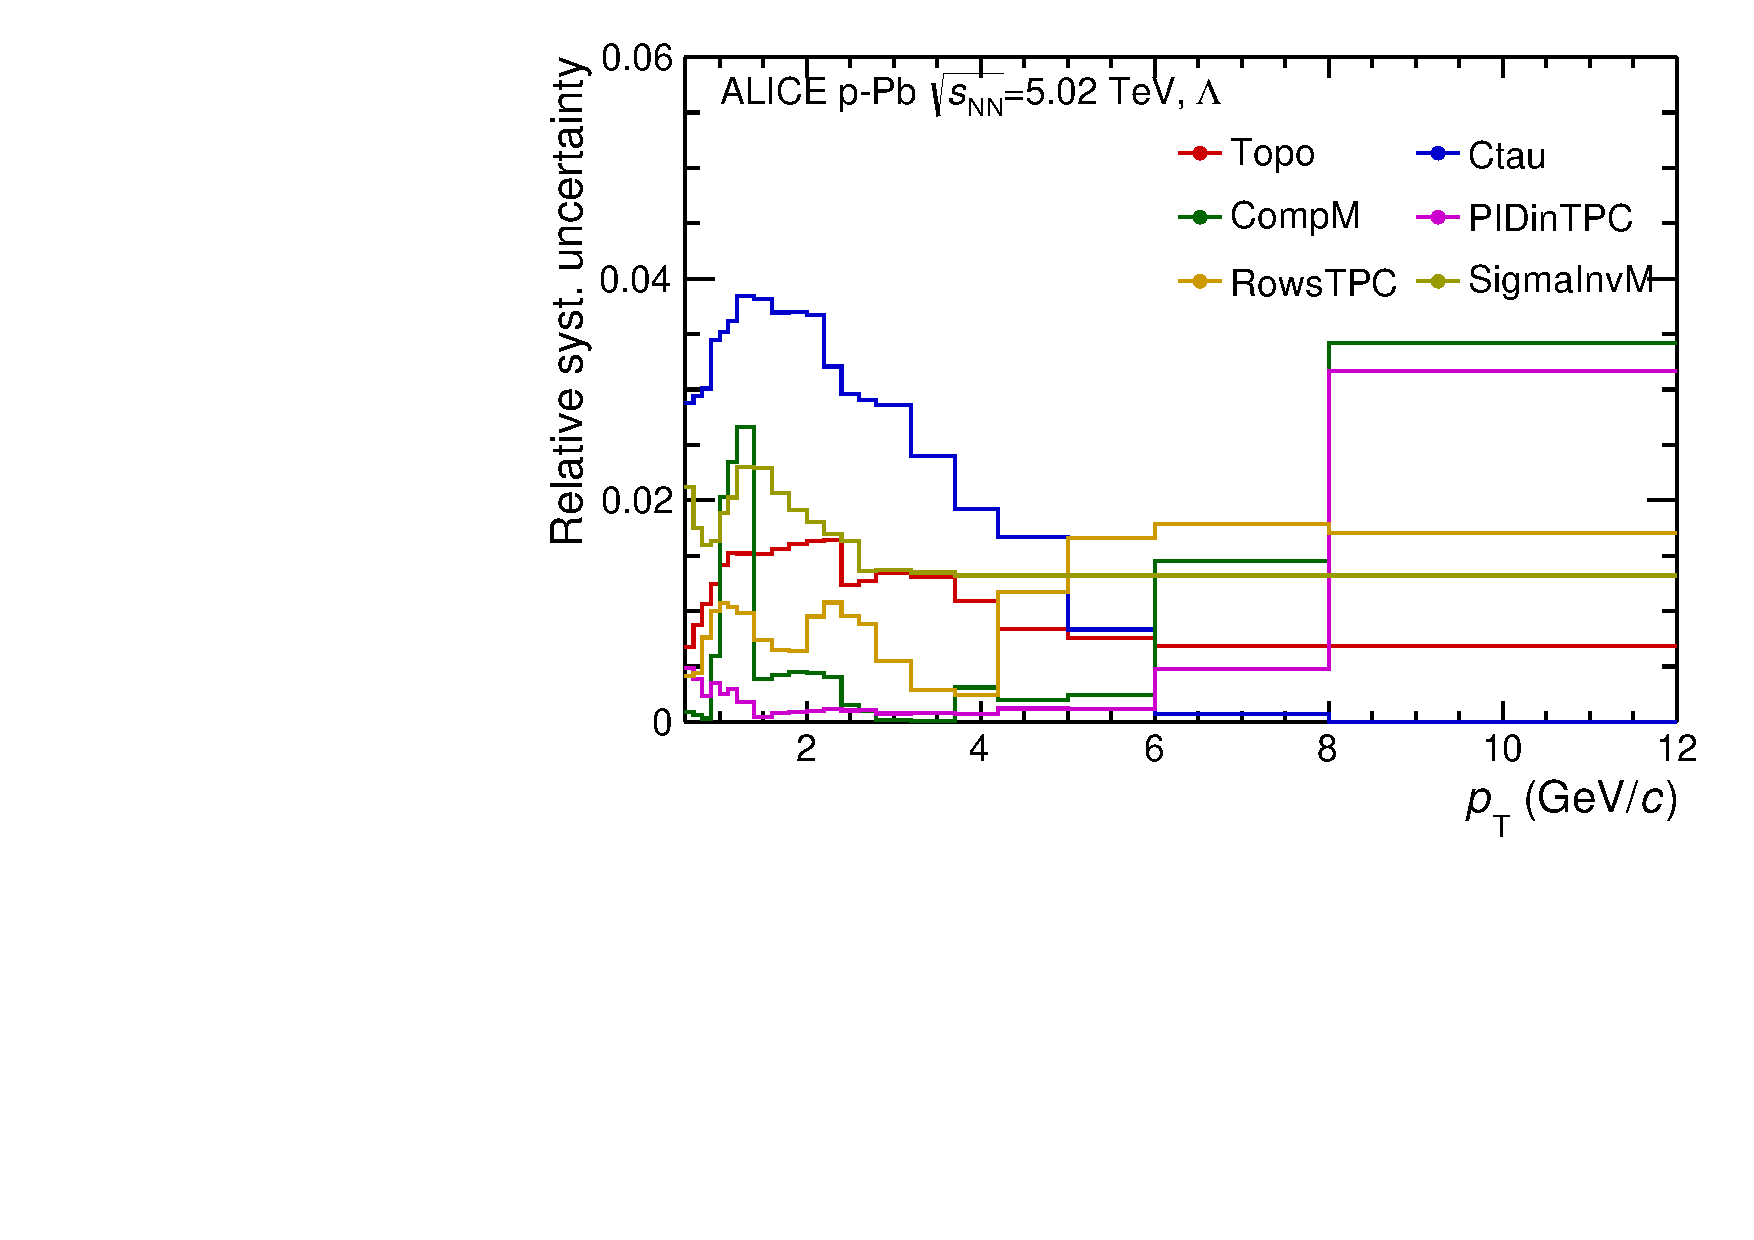
\includegraphics[width=.32\textwidth]{cCheckIncl_Lambda_Bin21}
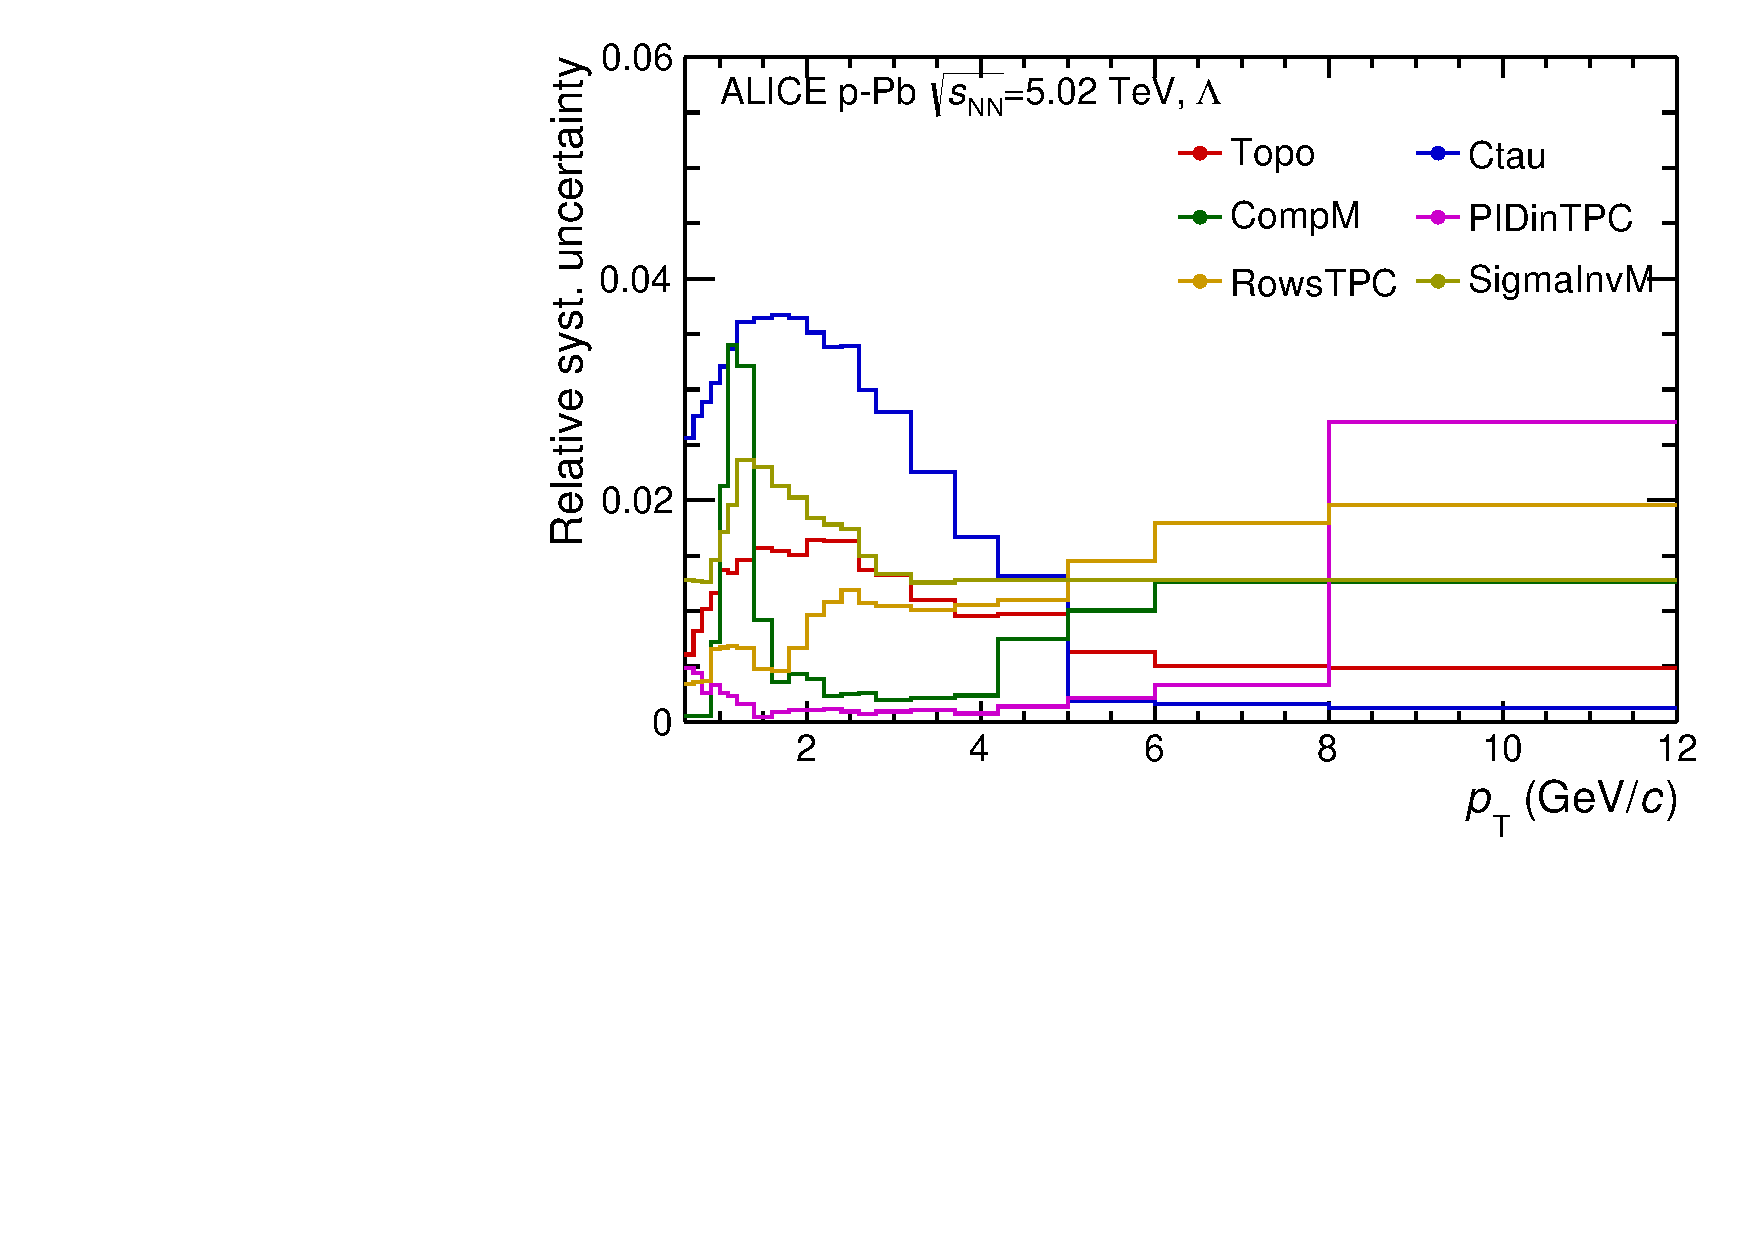
\includegraphics[width=.32\textwidth]{cCheckIncl_AntiLa_Bin21}
\caption{Updated uncertainty on $\Vzero$ yield of inclusive $\Vzero$s.}
\label{fig:NewInclSyst}
\end{figure}

%%%%%%%%%%%%%%%%%%%%%%%%%%%%%%

\bibliographystyle{utphys}
\bibliography{AliV0JetsPC20160712}

\end{document}